\chapter{Boolean Formulas and Equations}
\label{ch:Boolean-Formulas}

\section{Reasoning with Equations}
\label{sec:math-and-equations}
Symbolic logic, like other parts of mathematics, starts from a small
collection of axioms and employs rules of inference to find
additional propositions consistent with those axioms. This
chapter will define a grammar of logic formulas, specify a few
equations stating that certain formulas carry the same meaning as others,
and derive new equations
using substitution of equals for equals as the rule of
inference.

You will probably find this familiar from your
experience with numeric algebra, but the discourse here will attend carefully
to details, and this formality may extend beyond what you are
accustomed to. What it buys us is mechanization. That is,
logic formulas and reasoning about them will amount to
mechanized computation, and this will make it possible for
computers to check that our reasoning follows all the rules,
without exception. This provides a higher level of confidence
in conclusions than would otherwise be possible.

\begin{aside}
\emph{Hold on to your seat!}
This section illustrates an essential method used throughout the book.
It introduces the notion of ``formality'' in mathematics.
That is, formality in the sense of being based on formulas.
The formulas have a prescribed grammar similar to the one
for ordinary numeric formulas.
The grammar determines which formulas are well formed
(that is, grammatically correct) and which are not.
For example, ``$x+3\times(y + z)$'' conforms to the grammar
of numeric formulas,
so it is grammatically correct,
but the non-formula ``$x+3\times(y + ) \times z$'' is not.

Things may seem overly simple in the beginning.
Then, suddenly, you may find yourself thrashing around in deep water.
Take a deep breath, and slowly work  through the material.
It provides a basis for everything to follow.
The ideas and methods call for careful study and frequent review.
When things start to go off track,
just slow down, back up a little, and try again.
Gradually, the pieces will fall into place.
\caption{Hold on to Your Seat}
\label{aside-hold-on-to-seat}
\end{aside}

We will be doing all of this in the domain of symbolic logic, which
includes operations like ``logical or'' and ``logical negation'',
rather than arithmetic operations, such as addition and
multiplication.
We will be doing Boolean algebra, rather than numeric algebra, 
but the rule of inference that the reasoning is based on, 
namely substitution of equals for equals,
applies equally well to both Boolean and numeric formulas.
To illustrate the level of formality that we are shooting for,
let's see how it works with a problem 
in the familiar domain of numeric algebra.

You are surely familiar with the equation $(-1)\times(-1) = 1$, but you may
not know that it is a consequence of some basic facts about
arithmetic.
That is, the fact that multiplying two
negative numbers produces a positive one
is not independent of other facts about numbers.
Instead, it is an inference one can draw
from an acceptance of other familiar equations.
We will derived the equation $(-1)\times(-1) = 1$
from equations that you have accepted without question for a long time.

The equations in Figure~\ref{fig-02-01} (page \pageref{fig-02-01})
express some standard rules of numeric computation.
In those equations, the letters stand in
place of numbers. They can also stand in place of other
formulas.
So, the variable $x$ stands for a grammatically correct formula,
which could be something simple, such as ``$2$'',
it could be a more complicated formula, such as ``$3\times(y + 1)$''.

We refer to letters used in this way as
``variables'' even though, within a particular equation, they
stand for a fixed number or a particular formula.
The formula associated with a variable, though unspecified,
is the same for every occurrence of the variable in the equation.
That is, if $x$ stands for $3\times(y + 1)$ at one point in the
equation, then everywhere else $x$ occurs in the equation,
it stands for that same formula, $3\times(y + 1)$.
This is the usual custom in algebra.

\begin{figure}
\begin{center}
\begin{tabular}{ll}
$x+0 = x$                 & \{$+$ identity\} \\
$(-x)+ x = 0$             & \{$+$ complement\} \\
$x \times 1 = x$          & \{$\times$ identity\} \\
$x \times 0 = 0$          & \{$\times$ null\} \\
$x+y = y+x$               & \{$+$ commutative\} \\
$x \times y = y \times x$ & \{$\times$ commutative\} \\
$x+(y+z) = (x+y)+z$       & \{$+$ associative\} \\
$x \times (y \times z) = (x \times y) \times z$ & \{$\times$ associative\} \\
$x\times(y+z) = (x \times y)+(x \times z)$      & \{distributive law\} \\
\end{tabular}
\end{center}
\caption{Equations of Numeric Algebra}
\label{fig-02-01}
\end{figure}

If we accept the equations of Figure~\ref{fig-02-01} (page \pageref{fig-02-01}),
we can apply one of them to transform the formula $(-1)\times(-1)$ to a new formula that
stands for the same number. Then, we can apply another equation to
transform that formula to a new one, and so on. 
We look for a way to apply the
accepted equations one by one, so that in the end we
arrive at the formula ``1''. At every step, we know that the
new formula stands for the same value as the old one, so in
the end we know that $(-1)\times(-1) = 1$.

Figure~\ref{fig-02-02} (page \pageref{fig-02-02})
displays this sort of equation-by-equation derivation of the
formula ``1'' from the formula ``$(-1)\times(-1)$''. To
understand Figure~\ref{fig-02-02}, you must remember that each
variable can denote any
grammatically correct formula. For example, in the
\{$+$ identity\} equation, $x + 0 = x$, the variable $x$ could stand for
a number, such as 3, or it could stand for a more complicated
formula, such as $(1 + 3)$. It could even stand for a formula
with variables in it, such as $(a + (b \times c))$ or
$(((-1) \times (x + 3)) + (x + y))$.

Another crucial point is that each step cites
exactly one equation from Figure~\ref{fig-02-01} (page \pageref{fig-02-01})
to justify the transformation from the formula in the previous step.
We are so accustomed to calculating with numeric formulas that
we often combine many basic steps into one. When we reason formally,
we must not do this. We must justify each step by citing an equation
from a list of known equations. In our proof of $(-1)\times(-1) = 1$,
we will justify steps by citing equations from Figure~\ref{fig-02-01}
and from no other source. We will not skip steps.
Think of that as you go through the proof, line by line.

The first step in the proof
(Figure~\ref{fig-02-02}, page \pageref{fig-02-02}) uses a version of the
\{$+$ identity\} equation in which the variable $x$ stands for the
formula $((-1)\times(-1))$.
In this context, the \{$+$ identity\} equation 
leads to the new formula $((-1)\times(-1)) + 0$.

The second step in the proof reads the \{$+$ complement\}
equation backwards (equations go both ways), and in a form
where the variable $x$ stands for the number 1. 
When $x$ is 1, the \{$+$ complement\} equation is 
$(-1) + 1 = 0$. 
Reading the equation backwards, we can substitute
$((-1) + 1)$ for $0$,
and that leads to the formula $((-1)\times(-1)) + ((-1) + 1)$. 
So, we know now that
$(-1)\times(-1) = ((-1)\times(-1)) + ((-1) + 1)$.

Doesn't really seem like progress does it?
But, we press on anyway, one step at a time.
The transformations, step by step, finally confirm that the two formulas
$(-1)\times(-1)$ and 1 represent the same number.

Pay particular attention to the last three lines of the proof.
Most people tend to jump from the formula $0+1$ to the
formula $1$ in one step. That jump requires knowing the equation
$0+1 = 1$. However, that equation is not among those listed in
Figure~\ref{fig-02-01} (page \pageref{fig-02-01}).
We want to do the proof without citing any equations
other than those in Figure~\ref{fig-02-01}, so we need two steps
to get from ``$(0+1)$'' to ``$1$'',
and those are the last two steps in the proof.

\begin{figure}
\begin{center}
\begin{tabular}{lll}
    & $(-1)\times(-1)$                            & \\
$=$ & $((-1)\times(-1)) + 0$                      & \{$+$ identity\} \\
$=$ & $((-1)\times(-1)) + ((-1) + 1)$             & \{$+$ complement\} \\
$=$ & $(((-1)\times(-1)) + (-1)) + 1$             & \{$+$ associative\} \\
$=$ & $(((-1)\times(-1)) + ((-1) \times 1)) + 1$  & \{$\times$ identity\} \\
$=$ & $((-1)\times((-1) + 1)) + 1$                & \{distributive law\} \\
$=$ & $((-1)\times 0) + 1$                        & \{$+$ complement\} \\
$=$ & $0 + 1$                                     & \{$\times$ null\} \\
$=$ & $1 + 0$                                     & \{$+$ commutative\} \\
$=$ & $1$                                         & \{$+$ identity\} \\
\end{tabular}
\end{center}
\caption{Why $(-1)\times(-1)=1$}
\label{fig-02-02}
\end{figure}

One of the things we hope you will glean from this derivation is that
the equation $(-1)\times(-1) = 1$ does not depend on vague,
philosophical assertions like ``two negatives make a positive.''
Instead, the equation $(-1)\times(-1) = 1$ is a consequence of some
basic arithmetic equations. If you accept the basic equations
and the idea of substituting equals for equals, you must, as a
rational consequence, accept the equation $(-1)\times(-1) = 1$.

Using this same kind of reasoning, we will derive new Boolean equations
from a few, basic ones postulated as axioms.
A Boolean \emph{axiom} is a Boolean equation
that we assume to be true, without proof.
We will also learn that digital circuits are physical
manifestations of logic formulas, and we will be able to
parlay that idea to derive behavioral properties of
computer components.

Likewise, because a computer program is,
literally, a formula, we will be able to derive
properties of software directly from the programs, themselves. 
This makes it possible for us to be entirely
certain about some of the behavioral characteristics of
software, and of computer hardware, too,
since a hardware component is a physical embodiment of a formula
in logic.
Our certainty stems from the mechanistic
formalism that we insist on from the beginning,
which can be checked to the last detail with automated computation.

\begin{ExerciseList}
\label{ex:ch02-intro}
\Exercise
Use the equations of Figure~\ref{fig-02-01} (page \pageref{fig-02-01}),
together with the additional equation (1+1)=2, to derive the equation $(x + x) = (2 \times x)$.

\Exercise
Derive the following equation
using using the equations of Figure~\ref{fig-02-01}.
\begin{center}
\begin{tabular}{ll}
$((-1) \times x) + x = 0$    & \{$\times$ negation\}
\end{tabular}
\end{center}

\Exercise
Derive the equation $((x + (((-1) \times (x + y)) + z)) + y) = z$
using using the equations of Figure~\ref{fig-02-01} and,
if you like,
the \{$\times$ negation\} equation from the previous exercise.
\end{ExerciseList}

\section{Boolean equations}
\label{sec:boolean-equations}
Let's start with the Boolean equations in 
Figure~\ref{fig-02-03} (page \pageref{fig-02-03}).
These equations, which we will call the Boolean axioms,
are the starting point for our system of reasoning.
The form the basis from which we will derive
a host of other equations.
If these axiomatic equations are new to you and seem strange, 
try to view them as ordinary,
algebraic equations, but with a different collection of operators.
A formula in numeric algebra has operations like addition
($+$) and multiplication ($\times$). Boolean formulas employ logic
operations: logical-and ($\wedge$), logical-or ($\vee$),
logical-negation ($\neg$), and implication ($\rightarrow$).
Furthermore, Boolean formulas stand for logic values
($True$, $False$), rather than for numbers (\dots -2, -1, 0, 1, 2 \dots).

\begin{figure}
\begin{center}
\begin{tabular}{ll}
$x \vee False = x$                                   & \{$\vee$ identity\} \\
$x \vee True = True$                                 & \{$\vee$ null\} \\
$x \vee y = y \vee x$                                & \{$\vee$ commutative\} \\
$x \vee (y \vee z) = (x \vee y) \vee z$              & \{$\vee$ associative\} \\
$x \vee (y \wedge z) = (x \vee y) \wedge (x \vee z)$ & \{$\vee$ distributive\} \\
$x \rightarrow y = (\neg x) \vee y$                  & \{implication\} \\
$\neg(x \vee y) = (\neg x) \wedge (\neg y)$          & \{$\vee$ DeMorgan\} \\
$x \vee x = x$                                       & \{$\vee$ idempotent\} \\
$x \rightarrow x = True$                             & \{self-implication\} \\
$\neg(\neg x)  = x$                                  & \{double negation\} \\
\end{tabular}
\end{center}
\caption{Boolean Axioms (basic equations)}
\label{fig-02-03}
\end{figure}

When we derive new equations from equations we already know,
we refer to the derived equations as \emph{theorems} to
distinguish them from axioms. 
We call the derivation a
\emph{proof} of the theorem.

\begin{figure}
\begin{theorem}[\{$\vee$ truth table\}]
\mbox{}
\begin{itemize}
\item $False \vee False = False$
\item $False \vee True  = True$
\item $True  \vee False = True$
\item $True  \vee True  = True$
\end{itemize}
\end{theorem}

\begin{proof}
\mbox{}\\
\begin{tabular}{lll}
    &$False \vee False$    & \\
$=$ & $False$              & \{$\vee$ identity\}  ~~~---replace $x$ in the axiom with \emph{False}\\
    &  ~                   & \\
    & $False \vee True$    & \\
$=$ & $True$               & \{$\vee$ null\}  ~~~---replace $x$ in the axiom with \emph{False}\\
%    &                      & \dots for practice, prove the other two equations yourself \dots \\
\end{tabular}
\begin{quote}
\dots for practice, prove the other two equations yourself \dots
\end{quote}
\end{proof}
\caption{Proof of Theorem \{$\vee$ Truth Table\}}
\label{or-truth-table}
\end{figure}

The first equation in the theorem \{$\vee$ truth table\}
(Figure~\ref{or-truth-table}, page \pageref{or-truth-table})
is a special case of the
\{$\vee$ identity\} axiom (Figure~\ref{fig-02-03}),
and the proof of that equation simply amounts making that observation.
That is, the proof just rewrites the \{$\vee$ identity\} axiom
with $False$ in place of $x$.

The proof of the second equation is equally short, but cites
a different axiom.
For practice, try to prove the other two
equations in the \{$\vee$ truth table\} theorem
by citing axioms in a similar way.

We are serious about that. Did you prove the other two equations?
No? Well \dots go back and do it, then. Without participation, there
is no learning.

\smallskip
$\dots$ \emph{We'll wait here}$\dots$
\smallskip

Finished now? Good for you. You cited the \{$\vee$ identity\} axiom in your
proof of the third equation in the theorem and the \{$\vee$ null\}
axiom in your proof of the fourth equation, right? We knew you could do it.

\begin{aside}
A \emph{truth table} for a formula is a list of equations
stating the values the formula represents,
with one equation for every possible combination of values
of the variables in the formula.
If there is only one variable in the formula,
there will be two equations in its truth table,
one for the case when the variable has the value
$True$ and one for the case when the variable has the value $False$.
If there are two variables in the formula,
there will be four equations in the truth table
because for each choice of value for the first variable,
there are two choices for the other.
Three variables lead to eight equations.
The number of equations in the truth table
doubles with each additional variable
in the formula.

A truth table for a logic operator is the truth table for the formula
that has variables in place of the operands.
For example, the truth table for the logical-or operator ($\vee$)
is the truth table for the formula $(x \vee y)$.
That formula has two variables, so the truth table has four equations.
\caption{Truth Tables}
\label{truth-tables}
\end{aside}

Derivations are usually more than one step, of course.
For example, the
\{$\vee$ complement\} theorem
(Figure~\ref{fig:or-complement-thm}, page \pageref{fig:or-complement-thm})
has a two-step proof, citing the \{implication\} axiom
and the \{self-implication\} axiom.
The \{$\vee$ complement\} theorem is often called the
``law of the excluded middle'' because it says that any
logic formula, together with its negation, covers all
of the possibilities.
A formula in logic is either true of false.
There is no middle ground.

\begin{figure}
\begin{theorem}[\{$\vee$ complement\}]
$(\neg x) \vee x = True$
\end{theorem}
\begin{proof}
\mbox{}\\
\begin{tabular}{lll}
    & $(\neg x) \vee x$ & \\
$=$ & $x \rightarrow x$ & \{implication\} \\
$=$ & $True$            & \{self-implication\} \\
\end{tabular}

\end{proof}
\caption{Proof of Theorem \{$\vee$ complement\}}
\label{fig:or-complement-thm}
\end{figure}

All of the logic operators have truth tables,
and we can derive the equations in those truth tables from the axioms.
Figure~\ref{fig:neg-truth-table} (page \pageref{fig:neg-truth-table})
displays the truth table
for the negation operator $(\neg)$.
The figure includes a four-step proof of the first equation in
the table.
To beef up your comprehension of the ideas,
construct your own proof of the second equation in the theorem.

\begin{figure}
\begin{theorem}[\{$\neg$ truth table\}]
\mbox{}\\
\begin{itemize}
\item $\neg True = False$
\item $\neg False = True$
\end{itemize}
\end{theorem}
\begin{proof}
\mbox{} \\
\begin{tabular}{llp{3.15in}}
    & $\neg True$                      & \\
$=$ & $\neg (False \rightarrow False)$ & \{self-implication\} \\
$=$ & $\neg ((\neg False) \vee False)$ & \{implication\}     ---replace $x$ and $y$ in axiom with $False$ \\
$=$ & $\neg (\neg False)$              & \{$\vee$ identity\} ~~---replace $x$ in the axiom with $\neg False$ \\
$=$ & $False$                          & \{double negation\} ~~---replace $x$ in axiom with $False$ \\
\end{tabular}

\bigskip
\noindent
\begin{tabular}{lll}
    & $\neg False$                             & \\
$=$ & \dots you fill in the details here \dots & \\
$=$ & $True$                                   & \\
\end{tabular}

\end{proof}
\caption{Proof of Theorem \{$\neg$ truth table\}}
\label{fig:neg-truth-table}
\end{figure}

An important facet of these proofs is that they are
entirely syntactic. That is, they apply axioms by
matching the grammar of a formula $f$ (or a sub-formula of $f$) in the proof
with a formula $g$ from one side of an equation in the axioms.
The matching associates the variables in $g$ with corresponding sub-formulas of $f$.
Then, the formula $h$ on the other side of
the axiomatic equation is rewritten,
replacing each of variable in $h$ with the the associated subformula of $f$
that the matching process established.
The rewritten version of $h$
becomes the new, derived formula.
We know that the derived formula stands for the same value
as the original formula because the axiom asserts this equivalence,
and we are assuming that axioms are right.

\begin{aside}
Another way to prove that two formulas stand
for the same value is to build truth tables for both formulas.
A truth table lists all possible combinations of values for the
variables in a formula, and displays the value that the formula
denotes for each of those combinations. (Theorem \{$\vee$ truth table\} provides
the truth table for the logical-or operation, and theorem \{$\neg$ truth table\}
provides the truth table for the logical-negation operation.)
Two truth tables that list identical values of the corresponding
formulas for all combinations of values for
the variables demonstrate that the formulas always stand for the
same value. This proof method works well for formulas with only
a few variables. In that case, there are only a few combinations
of values for the variables, and the comparison can be completed quickly and accurately.

On the other hand, if there are many variables in the formulas,
things get out of hand. With two variables, as in the truth table
for logical-or, there are four combinations of values
(two choices for each variable, $True$ or $False$, so two times two
combinations in all). With three variables, there are eight
($2^3$) combinations, which makes the truth-table method tedious,
but not infeasible. After that, it gets rapidly out of hand.
Ten variables produce 1,024 ($2^{10}$) combinations of values.
That makes it difficult for people, but no real problem for a computer.
Even twenty variables (a little more than a million combinations)
also can be checked quickly by computers.

However, a formula specifying a computing component,
hardware or software, has hundreds of variables.
Our goal is to be able to reason about
computing components, and there is no hope of doing that
with truth tables when the formulas have hundreds of variables. 
The number of combinations
of values for the variables in a formula with, say,
100 variables is $2^{100}$, and that number is so large that no computer could
finish checking all the cases before the sun runs out of fuel,
so a straightforward appeal to truth tables is
definitely not feasible for formulas with lots of variables.

There are effective methods 
for dealing with at least some large formulas
besides the proofs that make up the core
material of this book.
Hardware and software designers sometimes use
SMT solvers (satisfiability modula theories) or
BDD tools (binary decision diagrams)
to verify properties of circuits and computer programs.
But, reasoning based on grammatical form
makes it possible to deal with formulas with any number of variables
because the formulas can be split into parts small enough
to manage, and those parts can be reintegrated, based on
their grammatical relationships, to produce a full analysis.
Feasible doesn't mean easy, though.
It usually takes a lot of effort,
but it can pay off.
\caption{Truth Tables and Feasibility}
\label{feasibility}
\end{aside}

Let's prove another truth-table theorem, partly to practice
reasoning with equations, but also to discuss a common
point of confusion about logic. The implication operator
($\rightarrow$) is a cornerstone of logic in real-world problems,
but it is common to get tripped up when it comes to
reasoning with implication.

The \{$\rightarrow$ truth table\} theorem
(Figure~\ref{implication-truth-table}, page \pageref{implication-truth-table})
provides the truth table
for the implication operator.
An important aspect of the proof is that it cites
not only axioms from Figure~\ref{fig-02-03} (page \pageref{fig-02-03}),
but also equations from the \{$\neg$ truth table\} theorem.
This is the way mathematics goes. Once we have derived
a new equation from the axioms, we can cite
the new equation to derive still more equations.

\begin{aside}
Citing proven theorems to prove new ones
is similar to an idea known as ``abstraction''
that is a mainstay in engineering design.
At the point where we cite an old theorem to prove a new one,
we could, instead, copy the proof of the old theorem into the new proof.
However, that would make the proof longer, harder to understand,
and more likely to contain errors than it would be if we had
applied the theorem instead of copying its proof.

Computer programs are built from components that are, themselves,
other computer programs. As a project proceeds, more and more
components become available, and they are used to build more complex ones.
Sometimes, a component has almost the right form to be used in a new program,
but not quite.
Maybe the existing component doubles a number where the new program would need
to triple it. It is tempting to make a copy the
old component and change the $2 \times x$ formula to $3 \times x$
at the point where a doubling should be a tripling,
then paste the revised component into the program.

In our experience
copy-and-paste programming is
a common cause of errors in software,
especially in big programs maintained,
over time, by many people, because
when a maintainer finds an error in
a section of code that was copied from elsewhere,
there is nothing to direct the maintainer to fix
the same error in the copied code.
A better choice, most of the time,
is to make a new component
in which the $2$ is replaced by a variable,
say $m$.

This is known as creating an ``abstraction'' of the component
(``abstract'' as opposed to ``specific'' or ``concrete'').
The new component can be used for both doubling and tripling,
simply by specifying $2$ for $m$ in one case and $3$ for $m$ in the other.
That way, if an error is discovered in the component later,
the error can be fixed in one place instead of two
(or maybe ten or a hundred places, depending on how many engineers
copied of the original component to make a change.

Abstraction is one of the most important methods in
all of engineering design. Citing old theorems to prove new ones,
instead of doing copy-and-paste with their proofs, 
is part of that tradition.
\caption{Abstraction}
\label{abstraction}
\end{aside}

\begin{figure}
\begin{theorem}[\{$\rightarrow$ truth table\}]
\mbox{}
\begin{itemize}
\item $False \rightarrow False = True$
\item $False \rightarrow True  = True$
\item $True  \rightarrow False = False$
\item $True  \rightarrow True  = True$
\end{itemize}
\end{theorem}

\begin{proof}
\mbox{} \\
\begin{tabular}{llp{3.15in}}
    & $False \rightarrow False$        & \\
$=$ & $(\neg False) \vee False$        & \{implication\} ~~---\emph{put} $False$ \emph{for} $x$ \emph{and for} $y$ \emph{in axiom}\\
$=$ & $\neg False$                     & \{$\vee$ identity\}\\
$=$ & $True$                           & \{$\neg$ truth table\}\\
\end{tabular}

\begin{tabular}{lll}
& \dots for practice, prove the other equations yourself\dots & \\
\end{tabular}

\end{proof}
\caption{Proof of Theorem \{$\rightarrow$ truth table\}}
\label{implication-truth-table}
\end{figure}

In day-to-day life outside the sphere of symbolic logic,
the usual interpretation of the logical implication ``$x \rightarrow y$''
is that we can conclude that $y$ is true if we know that
$x$ is true. However, the implication says nothing
about $y$ when $x$ is not true. In particular, it
does not say that $y$ is not true whenever $x$ is not true.
Theorem \{$\rightarrow$ truth table\} shows that the
formula ``$False \rightarrow y$'' has the value $True$ when $y$ is $True$
and also when $y$ is $False$.
In other words, the truth of the formula $x \rightarrow y$ in the case
where the hypothesis, $x$, of the implication is $False$ provides
no information about the conclusion, $y$.

A common mistake in everyday life is to assume that if the
implication ``$x \rightarrow y$'' is true, then the implication
``$(\neg x) \rightarrow (\neg y)$''
is also true. Sometimes this leads to bad
results, even in everyday life. In symbolic logic,
it is worse than that. Such a conclusion puts an
inconsistency into the mathematical system, and that renders the system useless.

Over half of the Boolean axioms in Figure~\ref{fig-02-03} (page \pageref{fig-02-03})
have names associated with the logical-or ($\vee$) operation.
One of them, the
\{$\vee$ DeMorgan\} equation
establishes a connection between logical-or and logical-and.
It converts the negation of a logical-or to the logical-and of two negations:
$\neg(x \vee y) = (\neg x) \wedge (\neg y)$.
We can use this connection to prove some logical-and equations
that are similar to the logical-or axioms.
An example is the null law for logical-and
(Figure~\ref{fig:and-null-thm}, page \pageref{fig:and-null-thm}).

\begin{figure}
\begin{theorem}[\{$\wedge$ null\}]
$x \wedge False = False$
\end{theorem}

\begin{proof}
\mbox{} \\
\begin{tabular}{llp{3.15in}}
    & $x \wedge False$                       & \\
$=$ & $x \wedge (\neg True)$                 & \{$\neg$ truth table\} \\
$=$ & $(\neg (\neg x)) \wedge (\neg True)$   & \{double negation\} \\
$=$ & $\neg ((\neg x) \vee True)$            & \{$\vee$ DeMorgan\} ~~---\emph{put} $(\neg x)$ \emph{for} $x$\emph{,} $True$ \emph{for} $y$ \emph{in axiom}\\
$=$ & $\neg True$                            & \{$\vee$ null\} \\
$=$ & $False$                                & \{$\neg$ truth table\} \\
\end{tabular}

\end{proof}
\caption{Proof of Theorem \{$\wedge$ null\}}
\label{fig:and-null-thm}
\end{figure}

This regime of theorem after theorem, proof after proof, is a little tiresome, isn't it?
Nevertheless, let's push through one more.
Then we'll give you a few to work out on your own, and go on to other topics.
We're not abandoning proofs, though.
Just taking a little break from proofs about equations.
It's going to be one proof after another, all the way down the line.

Some equations simplify the target formula when used in one direction,
but make it more complicated when used in the other direction.
For example, applying
the null law for logical-or, \{$\vee$ null\}, from left to right simplifies a logical-or formula to $True$.
When the equation is applied in the other direction, however,
it transforms the simple formula $True$ into something more complicated $(x \vee True)$.
The variable $x$ on the left-hand side
stands for any formula you want to make up (as long as it's grammatically correct).
It can have hundreds of variables and thousands operations.
This may seem perverse, but if that's what it takes to complete the proof, so be it.

The null law for logical-and, \{$\wedge$ null\}, is similarly asymmetric.
It goes from complicated to simple in one direction
and from simple to complicated in the other.
A particularly interesting and important asymmetric equation
is the absorption law for logical-and
(Figure~\ref{and-absorption-thm}, page \pageref{and-absorption-thm}).
It has two variables and two operations on one side, but only one variable and no operations on the other.

\begin{figure}
\begin{theorem}[\{$\wedge$ absorption\}]
$(x \vee y) \wedge y = y$
\end{theorem}

\begin{proof}
\mbox{} \\
\begin{tabular}{llp{3.15in}}
    & $(x \vee y) \wedge y$                & \\
$=$ & $(x \vee y) \wedge (y \vee False)$   & \{$\vee$ identity\} \\
$=$ & $(y \vee x) \wedge (y \vee False)$   & \{$\vee$ commutative\} \\
$=$ & $y \vee (x \wedge False)$            & \{$\vee$ distrubutive\} \\
$=$ & $y \vee False$                       & \{$\wedge$ null\} \\
$=$ & $y$                                  & \{$\vee$ identity\} \\
\end{tabular}

\end{proof}
\caption{Proof of Theorem \{$\wedge$ absorption\}}
\label{and-absorption-thm}
\end{figure}

We hope the gauntlet of theorems and proofs so far
(which we hope you have managed to get through, 
even if it took you to the point of exhaustion)
helps you understand how to derive a new equation from equations you already know.
The technique requires matching a formula to one side of a known equation,
then replacing it by the corresponding formula on the other side
of the equation.
The ``matching'' process is a crucial step.
It involves replacing the variables in the known equation
by constituents of the formula you are trying to match.
This is based in the mechanics of a formal grammar.
Unfortunately, it is surprisingly easy 
to have a lapse of concentration and make a mistake
while trying to substitute equals for equals.

Fortunately, it is easy for computers to verify
correct matchings and report erroneous ones.
A computer system that does this is known as a ``mechanized logic.''
After you have enough practice to gain a good understanding of the process,
we will begin to use a mechanized logic to make sure our reasoning is correct.

\begin{ExerciseList}
\Exercise
Use the Boolean axioms (Figure~\ref{fig-02-03}, page \pageref{fig-02-03})
and the $\wedge$-absorption theorem
(Figure~\ref{and-absorption-thm}, page \pageref{and-absorption-thm}),
to derive the $\vee$-absorption equation: $(x \wedge y) \vee y = y$.

\Exercise
Derive the equation
$(((\neg x) \wedge y) \vee (x \wedge (\neg y))) = ((x \vee y) \wedge (\neg(x \wedge y)))$
from the Boolean axioms.

\Exercise
Derive the equation
$(((\neg x) \wedge y) \vee (x \wedge (\neg y))) = (\neg((x \rightarrow y) \wedge (x \rightarrow y)))$
from the Boolean axioms.

\Exercise
Use the Boolean axioms
and the theorems of this section to
derive the truth-table for the following formula $(x \vee ((\neg y) \wedge (\neg z)))$.\\
\emph{Note}: Since there are three variables in the formula, the truth table
will have eight entries, and you will need to prove eight equations.
Each equation will have on the left-hand side
a different combination of values ($True$ or $False$) for the variables $x$, $y$, and $z$,
and on the right-hand side will have the value ($True$ or $False$) of the formula for that combination.
\end{ExerciseList}

\section{Boolean formulas}
\label{sec:boolean-formuas}

We have been doing proofs based on the grammatical elements of formulas,
but instead of taking the time to put together a precise definition of that grammar,
we have been relying on your experience with numeric algebra.
It is better to have a precise definition of the grammar,
starting with the most basic elements,
and working up from there to more complicated ones.

The simplest Boolean formulas are the basic constants ($True$ and $False$)
and variables ($x$, $y$, $\dots$). We normally use ordinary, lower-case letters,
for variables, but sometimes variables are letters with subscripts,
such as $x_3$, $y_i$, or $z_n$.
This gives us sufficient variety for any formula,
but we won't necessarily limit ourselves to lower-case, Roman letters.
We might use Greek letters, or
even make up recognizable squiggles, like Dr Seuss.

So, if you write $True$, $False$, or a letter from the alphabet,
you have composed a grammatically correct Boolean formula.
This is the first rule of Boolean grammar.
Formulas conforming to this rule have no substructure,
so we call them \emph{atomic} formulas.

Boolean operators make it possible to construct more complicated formulas.
We refer to operators that require two operands as \emph{binary operators }
($\wedge$, $\vee$, and $\rightarrow$).
These operators lead to the second rule of Boolean grammar:
If $a$ and $b$ are grammatically correct Boolean formulas,
 and $\circ$ is a binary operator
 (that is, $\circ$ is one of the symbols $\wedge$, $\vee$, or $\rightarrow$),
 then $(a \circ b)$ is also a grammatically correct Boolean formula.

For example, the first rule confirms that $x$ and $True$ are
grammatically correct Boolean formulas. Since $\wedge$ is a binary operator,
$(x \wedge True)$ is a grammatically correct Boolean formula by the
second rule of grammar. Furthermore, since $\rightarrow$ is a binary operator,
and $y$ is a grammatically correct Boolean formula (by the first rule),
$((x \wedge True) \rightarrow y)$ must be a grammatically correct
Boolean formula (by the second rule).

The third rule of Boolean grammar shows how to incorporate the negation operator into formulas.
The rule is that if $x$ is a grammatically correct formula, then so is $(\neg x)$.

These three rules are sufficient to
cover a full range of grammatically correct Boolean formulas,
and, they lead to an infinite variety of grammatically correct formulas.
However, there is a fine point to discuss about parentheses.
Parentheses are important because they make it easy to define
the grammar and to explain the meaning of a formula.
The formulas covered by the three rules are fully parenthesized,
including a top level of parentheses enclosing the entire formula
when an operator is involved.
Top level parentheses are often omitted in informal presentations,
and we have often omitted them.

For example, we have been writing formulas like ``$x \vee y$'',
without the top-level parentheses
the grammar requires.
To conform to the grammar,
we would have to write $(x \vee y)$, with the parentheses.
Because we have often omitted top-level parentheses,
requiring them probably comes as a surprise.
But, allowing non-atomic formulas without top-level parentheses
requires additional rules of grammar,
and we think that the added value of omitting parentheses
fails to compensate for the extra complexity.

Here is a more complex formula with incorrect grammar:
$x \wedge y \vee z$. This formula is missing two levels of parentheses.
Even worse, there are two options for the inner parentheses.
Does $x \wedge y \vee z$ mean $((x \wedge y) \vee z)$ or $(x \wedge (y \vee z))$?
There are ways to deal with formulas that omit parentheses,
but to avoid confusion, we are not going to allow such formulas.
The same problem occurs with formulas in numeric algebra.
We know that $x \times y + z$ means $((x \times y) + z)$ and
not $(x \times (y + z))$ because we know the convention that
gives multiplicative operators a higher precedence than additive operators.
But that takes some getting used to, and we want to
minimize the possibility of misinterpretation,
especially because Boolean formulas may be new to you.

We will sometimes be informal enough to omit
the top level of parentheses around the whole formula,
but we will not omit any interior parentheses.
The grammar does allow redundant parentheses, however.
For example, the formula $(x \vee ((x \wedge y)))$
is grammatically correct and has the same meaning as the formula
$(x \vee (x \wedge y))$.
The first formula has redundant parentheses,
but the second one doesn't.
Allowing redundant parentheses requires a fourth rule of grammar:
If $a$ is a grammatically correct Boolean formula, then so is $(a)$.

\begin{figure}
\begin{center}
\begin{tabular}{llll}
$v$             & \{atomic\}    &~~~~& \\
$(a \circ b)$   & \{bin-op\}    &~~~~& \emph{all grammatically correct formulas} \\
$(\neg a)$      & \{negation\}  &~~~~& \emph{~~~must match one of these templates}  \\
$(a)$           & \{group\}     &~~~~& \\
\end{tabular}

\vspace{2 mm}

\emph{requirements on symbols}

\begin{tabular}{l}
\hline
$\bullet$ ~~ $v$ is a variable or $True$ or $False$ \\
~~~~~(a variable is a letter or a letter with a subscript) \\
$\bullet$ ~~ $a$ and $b$ are grammatically correct Boolean formulas \\
$\bullet$ ~~ $\circ$ is a binary operator \\
\hline
\end{tabular}
\end{center}
\caption{Rules of Grammar for Boolean Formulas}
\label{fig-02-grammar}
\end{figure}

\begin{figure}
\begin{center}
\begin{tabular}{ll}
$(x \vee False) = x$                                     & \{$\vee$ identity\} \\
$(x \vee True) = True$                                   & \{$\vee$ null\} \\
$(x \vee y) = (y \vee x$)                                & \{$\vee$ commutative\} \\
$(x \vee (y \vee z)) = ((x \vee y) \vee z)$              & \{$\vee$ associative\} \\
$(x \vee (y \wedge z)) = ((x \vee y) \wedge (x \vee z))$ & \{$\vee$ distributive\} \\
$(x \rightarrow y) = ((\neg x) \vee y)$                  & \{implication\} \\
$(\neg(x \vee y)) = ((\neg x) \wedge (\neg y))$          & \{$\vee$ DeMorgan\} \\
$(x \vee x) = x$                                         & \{$\vee$ idempotent\} \\
$(x \rightarrow x) = True$                               & \{self-implication\} \\
$(\neg(\neg x))  = x$                                    & \{double negation\} \\
$((x)) = (x)$                                            & \{redundant grouping\} \\
$(v) = v$                                                & \{atomic release\} \\
\end{tabular}

\vspace{2 mm}

\emph{requirements on symbols}

\begin{tabular}{l}
\hline
$\bullet$ ~~ $x$, $y$, and $z$ are grammatically correct Boolean formulas \\
$\bullet$ ~~ $v$ is a variable or $True$ or $False$ \\
~~~~~(a variable is a letter or a letter with a subscript) \\
\hline
\end{tabular}
\end{center}
\caption{Axioms of Boolean Algebra}
\label{fig-02-boolean-axioms}
\end{figure}

With the four rules of 
Figure~\ref{fig-02-grammar} (page \pageref{fig-02-grammar}),
we can determine whether or not any given sequence of symbols 
is a grammatically correct Boolean formula.
The definition of the grammar is circular, 
but in a useful way that shows 
how to build more complicated formulas from simpler ones.

To verify that a formula is grammatically correct, 
find the rule of grammar that matches it, 
then verify that each part of the formula 
that matches with a variable in the rule of grammar 
is also grammatically correct. 
Atomic formulas have no substructure, 
so they require no further analysis when checking for grammatical correctness.

For example, consider the formula 
$((x \vee (\neg y)) \wedge (x \rightarrow z))$. 
It matches with the \{bin-op\} rule. 
The variables in the rule match 
with the elements of the formula in the following way.
\begin{center}
\begin{tabular}{ll}
\emph{symbol from \{bin-op\} rule}      & \emph{matching element in} $((x \vee (\neg y)) \wedge (x \rightarrow z))$ \\
$a$                                     & $(x \vee (\neg y))$ \\
$\circ$                                 & $\wedge$ \\
$b$                                     & $(x \rightarrow z)$ \\
\end{tabular}
\end{center}

The only other symbols in the rule are the top-level parentheses, and these match identically with the outer parentheses in the target formula. Therefore, the target formula is grammatically correct if the formulas $(x \vee (\neg y))$ and $(x \rightarrow z)$  are grammatically correct. We use the same approach to verify the grammatical correctness of those formulas.

The first one, $(x \vee (\neg y))$, 
again matches with the \{bin-op\} rule,
but this time the matchings of the elements 
in the target formula with variables in the rule are as follows:
\begin{center}
\begin{tabular}{ll}
\emph{symbol from \{bin-op\} rule}      & \emph{matching element in}  $(x \vee (\neg y))$ \\
$a$                                     & $x$ \\
$\circ$                                 & $\vee$ \\
$b$                                     & $(\neg y)$ \\
\end{tabular}
\end{center}

This reduces the verification of the grammatical correctness of $(x \vee (\neg y))$
to the verification of the two formulas $x$ and $(\neg y)$.
Since $x$ matches with the \{atomic\} rule, it must be grammatically correct.
The $(\neg y)$ element matches with the \{negation\} rule,
with $y$ from the formula matching $a$ in the rule.
So, $(\neg y)$ is grammatically correct if $y$ is,
and $y$ is grammatically correct because it matches with the \{atomic\} rule.
That completes the verification that the $(x \vee (\neg y))$ formula is grammatically correct.

The second element of the original formula,
$(x \rightarrow z)$, is easier to verify.
It matches the \{bin-op\} rule with $x$ corresponding to $a$ in the rule,
$y$ corresponding to $b$, and $\rightarrow$ corresponding to $\circ$ in the rule.
Since $x$ and $z$ match the \{atomic\} rule, they are grammatically correct.
This completes the verification of the grammatical
correctness of the formula $((x \vee (\neg y)) \wedge (x \rightarrow z))$.

Let's look at another example: $(x \vee (\wedge y)$. 
This sequence of symbols matches with the \{bin-op\} rule, 
with $x$ corresponding to $a$ in the rule, 
$\vee$ corresponding to $\circ$, 
and $(\wedge y)$ corresponding to $b$. 
So, the formula is grammatically correct 
if $x$ and $(\wedge y)$ are. 
However, there is no rule that matches $(\wedge y)$. 
The only place the symbol $\wedge$ could match a rule 
in the table is in the \{bin-op\} rule. 
In the \{bin-op\} rule, there must be 
a grammatically correct formula between 
the opening parenthesis and the operator. 
Since there is no such element present 
between the opening parenthesis 
and the $\wedge$ operator in the target formula, 
it cannot be grammatically correct.

That covers the grammar of Boolean formulas. 
What about meaning? 
Every grammatically correct Boolean formula denotes, 
when the values of its variables are specified, 
either the constant $True$ or the constant $False$. 
Each of the binary operators, given specific operands ($True$ or $False$), 
delivers a specific result ($True$ or $False$). 
We worked out what values the operators deliver 
when we derived truth-table theorems for them 
(as in Figure~\ref{or-truth-table}, page \pageref{or-truth-table}, for example).

In the process of deriving the truth tables,
we used the Boolean axioms of 
Figure~\ref{fig-02-03} (page \pageref{fig-02-03}).
We can use this same method to derive the meaning 
of any grammatically correct formula that contains no variables. 
However, to deal with parentheses in a completely mechanized way, 
we need to add two equations to those of Figure~\ref{fig-02-03}. 
The axioms of Figure~\ref{fig-02-boolean-axioms} (page \pageref{fig-02-boolean-axioms})
provides all of the information needed to determine 
the value of any grammatically correct formula 
that contains no variables. 
In fact the equations in the figure have even more general applicability. 
They provide all the information needed 
to verify not only whether a given formula 
has the same meaning as the formula $True$ or the formula $False$, 
but also to verify whether or not any two given, 
grammatically correct, formulas have the same meaning.

\begin{ExerciseList}

\Exercise Use the rules of grammar for Boolean formulas (Figure~\ref{fig-02-grammar}, page \pageref{fig-02-grammar})
to determine which of the following formulas are grammatically correct.
\begin{center}
\begin{tabular}{l}
$((x \wedge y) \vee y )$ \\
$((x \rightarrow y) \wedge (x \rightarrow (\neg y)))$ \\
$((False \rightarrow (\neg y)) \neg (x \vee True))$ \\
\end{tabular}
\end{center}


\Exercise Derive the truth tables (see page \pageref{truth-tables})
of the formulas from the previous exercise.

\Exercise Use the axioms of Boolean algebra
(Figure~\ref{fig-02-boolean-axioms}, page \pageref{fig-02-boolean-axioms})
to prove the equations in
Figure~\ref{some-boolean-theorems} (page \pageref{some-boolean-theorems}).\\
\emph{Note}: After proving an equation, you may cite it in subsequent proofs.

\end{ExerciseList}

\begin{figure}
\begin{center}
\begin{tabular}{ll}
$(x \rightarrow False) = (\neg x)$                                   & \{$\neg$ as $\rightarrow$\}\label{neg-as-imp} \\
$(\neg(x \wedge y)) = ((\neg x) \vee (\neg y))$                      & \{$\wedge$ DeMorgan\}      \label{and-DeMorgan} \\
$(x \vee (\neg x)) = True$                                           & \{$\vee$ complement\}      \label{or-complement} \\
$(x \wedge (\neg x)) = False$                                        & \{$\wedge$ complement\}    \label{and-complement} \\
$(\neg True) = False$                                                & \{$\neg True$\}            \label{not-True} \\
$(\neg False) = True$                                                & \{$\neg False$\}           \label{not-False} \\
$(True \rightarrow x) = x$                                           & \{$\rightarrow$ identity\} \label{imp-identity} \\
$(x \wedge True) = x$                                                & \{$\wedge$ identity\}      \label{and-identity} \\
$(x \wedge y) = (y \wedge x)$                                        & \{$\wedge$ commutative\}   \label{and-commutative} \\
$(x \wedge (y \wedge z)) = ((x \wedge y) \wedge z)$                  & \{$\wedge$ associative\}   \label{and-associative} \\
$(x \wedge (y \vee z)) = ((x \wedge y) \vee (x \wedge z))$           & \{$\wedge$ distributive\}  \label{and-distributive} \\
$(x \wedge x) = x$                                                   & \{$\wedge$ idempotent\}    \label{and-idempotent} \\
$(x \rightarrow y) = ((\neg y) \rightarrow (\neg x))$                & \{contrapositive\}         \label{contrapositive} \\
$(x \rightarrow (y \rightarrow z)) = ((x \wedge y) \rightarrow z)$   & \{Currying\}               \label{currying} \\
$((x \wedge y) \vee y) = y$                                          & \{$\vee$ absorption\}      \label{or-absorption} \\
$((x \rightarrow y) \wedge (x \rightarrow z)) = (x \rightarrow (y \wedge z))$ & \{$\wedge$ implication\} \label{and-implication} \\
$((x \rightarrow y) \wedge (x \rightarrow (\neg y))) = (\neg x)$     & \{absurdity\}              \label{absurdity} \\
$(x \rightarrow (\neg x)) = (\neg x)$                                & \{contradiction\}          \label{boolean-contradiction} \\
\end{tabular}
\end{center}
\caption{Some Boolean Theorems}
\label{some-boolean-theorems}
\end{figure}

\section{Digital Circuits}

Logic formulas provide a mathematical notation for concepts in symbolic logic.
These same concepts can be materialized as electronic devices.
The basic operators of logic represented in the form of electronic devices
are called ``logic gates''.
There are logic gates for the logical-and, the logical-or, negation, and
several other operators that we have not yet discussed.

\begin{aside}
One of the operators we have discussed at length, implication
($\rightarrow$), is not among the operators normally represented
in the form of logic gates. This does not restrict the kinds of
operations that can be performed by digital logic because,
as we know from the \{implication\} axiom of Boolean algebra
(Figure~\ref{fig-02-boolean-axioms}, page \pageref{fig-02-boolean-axioms}),
the formula $(x \rightarrow y)$ has the same meaning as the
formula $((\neg x) \vee y)$. So, anything we can do with
the implication operator, we can also with
negation and logical-or.

The lack of a conventional logic gate for the implication operator
is ironic.
George Boole himself, the inventor of Boolean algebra,
called implication the queen of logic operators.
It is one of only a few basic operators
that are \emph{functionally complete} in the sense that,
for any formula in logic, there is an equivalent formula
with no operators other than implication.
That is, given any grammatically correct logic formula,
there is a formula using only
implication operators (no logical-and, logical-or,
negation, or any other operators)
that has the same meaning.
Logical-or and logical-and are not functionally complete.
However, their negations, \emph{nor} and \emph{nand}, are.
For that reason nor gates and nand gates
are called \emph{universal gates}.
Figure~\ref{fig-02-nand-is-all-you-need} (page ~\pageref{fig-02-nand-is-all-you-need})
shows how to write logic formulas using only nand gates.

It is possible that implication gates may
become common in digital circuits in the future
because there is a way to fabricate implication gates that may allow extensive,
three-dimensional stacking of circuits, which up to now has been infeasible.
If that pans out, it could be possible to build
faster circuits with more components in a smaller space.
R. Stanley Williams discusses this
idea in an interesting video on ``memristor chips''
(\url{http://www.youtube.com/watch?v=bKGhvKyjgLY}).
\caption{Implication Gate Is Universal}
\label{no-implication-gate}
\end{aside}

A logic gate takes input signals that correspond
to the operands of logic operators and delivers output signals
that correspond to the values delivered by those operators.
A logic gate with two inputs is a physical representation of
a binary operator. The negation operator corresponds to a
logic gate with one input.

Logic operands and values are always either $True$ or $False$.
Similarly, an input line of a logic gate can distinguish between
only two distinct signals
and deliver only two distinct signals on an output line.
Conventionally those signals are written as 1 (for $True$) and 0 (for $False$).
Of course, logic gates are electronic devices,
so 1 and 0 are just labels for the signals.
Any two different symbols could be used to represent them in writing.
The choice of 1 and 0 is more-or-less arbitrary.

There are many ways to handle the electronics,
but we are going to leave the physics to the electrical engineers.
You can imagine representing the signal 1 as
a voltage at a point in a circuit and the signal 0 as
the lack a voltage, which is the way some technologies
deal with logic signals,
but we are going to focus on the logic and trust that
the electronic hardware can faithfully deal with
a signal representing $True$ and a different one representing $False$.

Circuits can be depicted as wiring diagrams
in which ``wires'' (represented by lines) carry signals between gates.
Distinctive shapes in the diagrams represent different logic gates.
Circuits can be represented as formulas as well as diagrams, and
the logic formulas we have been using would serve the purpose,
but traditionally the algebraic notation for circuits takes a
different form.
The algebraic notation commonly used by circuit
designers represents the logical-and by the juxtaposition
of the names being used for the input signals (in the same way
that juxtaposition of variables is used to denote multiplication
in numeric algebra). Logical-or is represented by a plus sign (+),
and negation is represented by a bar over the formula being negated
For example, the formula $\overline{ab}$ denotes the negation of the logical-and
of the signals $a$ and $b$.

\begin{figure}
\begin{center}
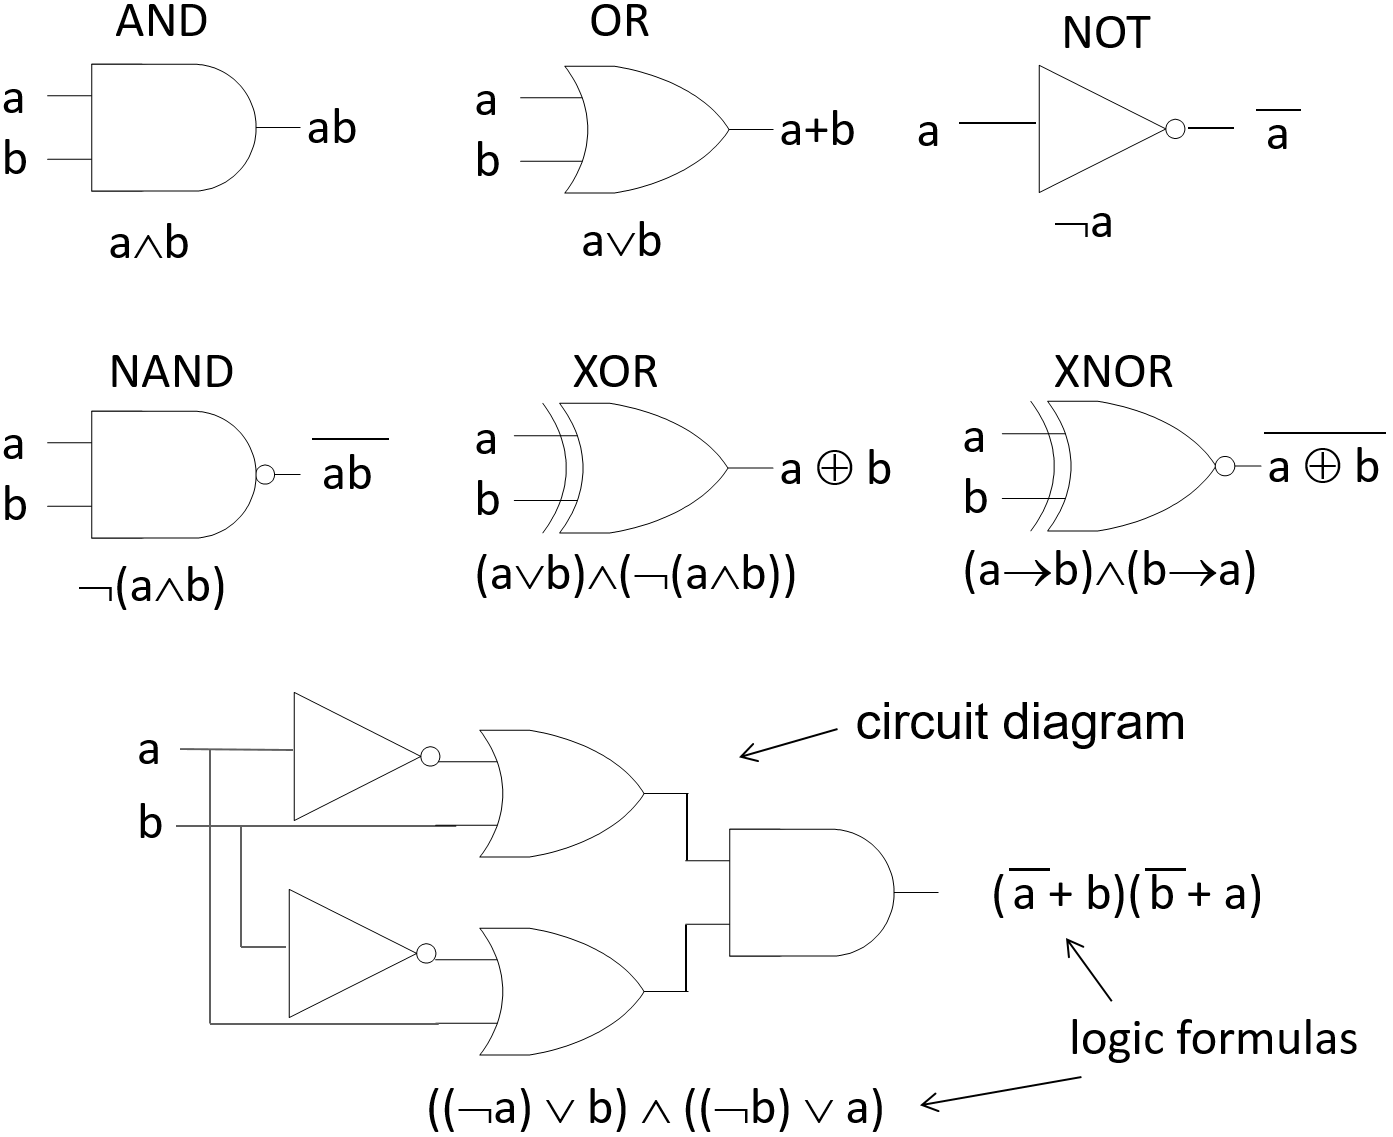
\includegraphics[scale=0.25]{images/LogicGates.png}
\todo{I did not have Visio with me. Improvised with PowerPoint. Figure will need to be redrawn.}
\end{center}
\caption{Digital Circuits = Logic Formulas}
\label{fig-02-logic-gates}
\end{figure}

Figure~\ref{fig-02-logic-gates} (page \pageref{fig-02-logic-gates})
presents the symbols used for logic gates in circuit diagrams
and annotates them with both
the algebraic notation used by circuit designers
and the logic formulas we have been using.
The important fact to remember is that all three notations
represent the same concepts in logic. Circuit diagrams, logic formulas,
and the algebraic notation used by circuit designers are three
different notations for exactly the same mathematical objects.
In this sense, digital circuits, and, therefore, computers,
are materializations of logic formulas.
Computers are logic in action.

The logic operators that we have been using
($\wedge$, $\vee$, $\neg$, $\rightarrow$)
make it possible to write a formula
the delivers precisely the values in the truth table
for any given formula.
The \{implication\} axiom
(Figure~\ref{fig-02-boolean-axioms}, page \pageref{fig-02-boolean-axioms})
expresses implication in terms of logical-and, logical-or,
and negation, which means we lose no expressive power by
discarding implication from the set of logic operations.

Surprisingly, the reverse is also true.
That is, for any given input/output relationship that can be expressed
in a formula using logical-and, logical-or, and negation,
there is a logic formula using implication as
the only operator that has the same input/output relationship.
The \{$\neg$ as $\rightarrow$\} equation
(Figure~\ref{some-boolean-theorems}, page \pageref{some-boolean-theorems})
provides a start in this direction by showing how to express
negation in terms of the implication operator.
Furthermore, implication is not the only logic operator
that is universal in this sense.
Another one
is the negation of logical-and, which is called ``nand''.
Many digital systems make frequent use of
nand gates because they can run faster and be more reliable
when fabricated with some widely used technologies 
for making integrated circuits.

It is interesting to see how to put together digital
circuits for basic operators.
$\wedge$, $\vee$, and $\neg$, using only nand gates.
Consider negation, for example.
Negation has only one input signals, and nand has two.
Feeding the same signal into both
inputs of a nand gate produces the behavior of
the negation operator,
as expressed in the following equation.

\begin{center}
\begin{tabular}{ll}
$(\neg a) = (\neg (a \wedge a))$  & \{$\neg$ as nand\}\label{neg-as-nand}
\end{tabular}
\end{center}

In this way a nand gate can serve in place of a
negation gate (also known as an inverter).
There is a one-step proof of the equation,
citing the \{$\wedge$ idempotent\} theorem
(page \pageref{and-idempotent}).

A nand-only circuit for logical-and can be
put together from two nand gates in sequence.
The signal from the first nand gate is inverted
by feeding it into both inputs of a second nand gate.
Algebraically, this circuit corresponds to the following \{$\wedge$ as nand\} equation.
It takes a two-step proof to verify the equation.
The first step converts the outside nand to negation using the
\{$\neg$ as nand\} equation, and the second step cites
the \{double negation\} axiom from Figure~\ref{fig-02-boolean-axioms}
(page \pageref{fig-02-boolean-axioms}).

\begin{center}
\begin{tabular}{ll}
$(a \wedge b) = (\neg ((\neg (a \wedge b)) \wedge (\neg (a \wedge b))))$ & \{$\wedge$ as nand\}\label{and-as-nand}
\end{tabular}
\end{center}

Negation took one nand gate and
logical-and took two.
Logical-or can be implemented with three nand gates,
as shown in the following equation,
which can be verified using
the \{$\neg$ as nand\} equation, DeMorgan's laws,
and double negation.

\begin{center}
\begin{tabular}{ll}
$(a \vee b) = (\neg ((\neg(a \wedge a)) \wedge (\neg(b \wedge b))))$ & \{$\vee$ as nand\}\label{or-as-nand}
\end{tabular}
\end{center}

Figure~\ref{fig-02-nand-is-all-you-need} (page \pageref{fig-02-nand-is-all-you-need})
diagrams the digital circuits
corresponding to the formulas that express logical-and, logical-or, and negation
in terms of nand operations.

\begin{figure}
\begin{center}
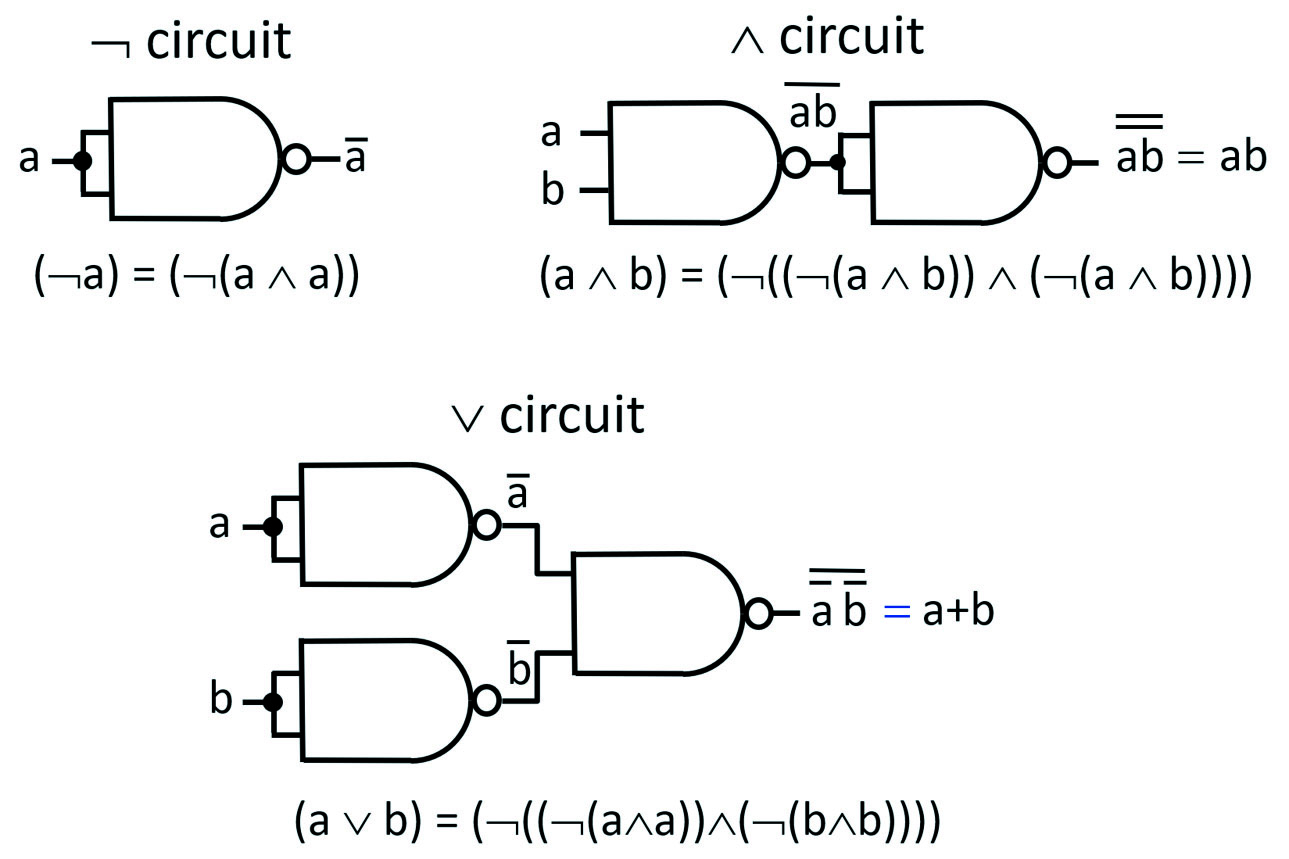
\includegraphics[scale=0.27]{images/NandIsAllYouNeed.png}
\todo{I did not have Visio with me. Improvised with PowerPoint. Figure will should be redrawn.}
%% redrew diagram ... still used PowerPoint, but improved the diagram a little 8Aug2017
\end{center}
\caption{Nand is All You Need}
\label{fig-02-nand-is-all-you-need}
\end{figure}

\begin{ExerciseList}
\Exercise Using a negation-gate and an or-gate, draw a circuit diagram with the input/output behavior of the implication operator.
We refer to this circuit diagram as an ``implication circuit''.\\
\emph{Hint}: Follow the example of the \{implication\} axiom
(Figure~\ref{fig-02-boolean-axioms}, page \pageref{fig-02-boolean-axioms})).
One of the inputs will need to be a constant rather than a variable.

\Exercise For each of the following logic formulas, draw an equivalent circuit diagram.
Since we don't have a symbol for an implication gate,
you can either make up you own symbol or
materialize logic gates where you need them
using the circuit diagram from the previous exercise.
\begin{center}
\begin{tabular}{l}
$((a \vee (b \wedge (\neg a))) \vee (\neg (a \vee b)))$ \\
$(((\neg a) \wedge (\neg b)) \wedge (b \wedge (\neg c)))$ \\
$(a \rightarrow (b \rightarrow c))$ \\
$((a \wedge b) \rightarrow c)$ \\
\end{tabular}
\end{center}

\Exercise Rewrite each of the formulas in the previous exercise
in the algebraic notation used by electrical engineers:
juxtaposition for $\wedge$, + for $\vee$, and $\overline{a}$ for $(\neg a)$.
Use the \{implication\} axiom to represent
implications using negation and logical-or.

\Exercise Draw circuit diagrams with behavior
of the and gate, the or gate, and the negation gate
using implication operators only.
\end{ExerciseList}

\todo{ do we still want to add half-adder and/or full-adder
circuits as examples? problem: they have two outputs, so need to talk about
tapping outputs from subformulas to show correspondence to algebraic form}

\section{Deduction}

We have been reasoning with equations, which means we are reasoning in two directions
at the same time, since equations go both ways. Deductive reasoning is one-directional.
It derives a conclusion from hypotheses using one-directional rules of inference.
A proof shows that the conclusion is true whenever the hypotheses are true, but provides
no information about the conclusion when the truth of one or more of the hypotheses is
unknown.

In the following discussion of proof by deduction,
theorems will be stated using the symbol ``$\vdash$'',
which is called a turnstile, to separate the hypotheses from the conclusions.
Hypotheses go on the left of the turnstile and the conclusion goes on the right.
All of the hypotheses are formulas in logic, as is the conclusion.
A theorem asserts that there is a derivation of the conclusion
from the hypotheses using the rules of inference.
The commutativity law for logical-and, for example,
can be stated as follows.
\begin{center}
Theorem \{$\wedge$ commutes\}: $a \wedge b \vdash b \wedge a$
\end{center}

Later, we will prove this theorem using a formal apparatus
for deductive reasoning known as
\emph{natural deduction}.\footnote{Natural
deduction is a formal system of logic pioneered in the 1930s
by the mathematician, Gerhard Gentzen, and refined in the 1960s
by the logician, Dag Prawitz.}
A deductive proof of a theorem with hypothesis $h$ and conclusion $c$
verifies that the implication $(h \rightarrow c)$ is true:
\begin{center}
$h \vdash c$ ~~ensures that~~ $(h \rightarrow c) = True$
\end{center}

\begin{figure}
\begin{center}
\begin{tabular}{ll}
Prove $a$                                               & Prove $a \vee b$                                  \\
 - - - - - -                                            &  - - - - - - - - - -                              \\
Prove $b$                                               & Prove $a \rightarrow c$                           \\
--------------\{$\wedge$ introduction\}                 &  - - - - - - - - - -                              \\
Infer $a \wedge b$                                      & Prove $b \rightarrow c$                           \\
                                                        & -----------------\{$\vee$ elimination\}           \\
                                                        & Infer $c$                                         \\
Prove $a$                                               &                                                   \\
--------------\{$\vee$ introduction 1\}                 &                                                   \\
Infer $a \vee  b$                                       & Prove $a \wedge b$                                \\
                                                        & ----------------\{$\wedge$ elimination 1\}        \\
                                                        & Infer $a$                                         \\
Prove $b$                                               &                                                   \\
--------------\{$\vee$ introduction 2\}                 &                                                   \\
Infer $a \vee  b$                                       & Prove $a \wedge b$                                \\
                                                        & ----------------\{$\wedge$ elimination 2\}        \\
                                                        & Infer $b$                                         \\
Prove $a \rightarrow False$                             &                                                   \\
-----------------------\{$\neg$ introduction\}          &                                                   \\
Infer $\neg a$                                          & Prove $\neg a$                                    \\
                                                        & ---------------------\{$\neg$ elimination\}       \\
                                                        & Infer $a \rightarrow False$                       \\
Prove $a$                                               &                                                   \\
----------\{identity\}                                  &                                                   \\
Infer $a$                                               & Prove \emph{False}                                \\
                                                        & ---------------\{contradiction\}                  \\
                                                        & Infer $a$                                         \\
Prove $a$                                               &                                                   \\
 - - - - - - - - - -                                    &                                                   \\
Prove $a \rightarrow b$                                 & Prove $(\neg a) \rightarrow$ \emph{False}         \\
-----------------\{modus ponens\}                       & --------------------------\{reductio ad absurdum\}\\
Infer $b$                                               & Infer $a$                                         \\
                                                        &                                                   \\
\end{tabular}
\end{center}
\begin{center}
\begin{tabular}{ll}
Assume $a$                                      & \emph{assumption required to cite} \{$\rightarrow$ introduction\}     \\
--------------\{\emph{r}\}                      & \emph{r is an inference rule or proven theorem}                       \\
Prove $b$                                       & $b$ \emph{has now been derived from assumption} $a$                   \\
-----------------\{$\rightarrow$ introduction\} & \emph{proof above line begins with} ``Assume \emph{left operand''}    \\
Infer $a \rightarrow b$                         & ~~~~\emph{and concludes with right operand, proving} $a \rightarrow b$\\
Discharge $a$                                   & \emph{excludes formula} ``$a$'' \emph{from hypotheses of theorem}     \\
\end{tabular}
\end{center}
\caption{Rules of Inference for Natural Deduction}
\label{fig-02-deduction-rules}
\end{figure}

Of course the truth of an implication formula doesn't
say anything about the value of the
left-hand operation of the implication operator.
That value could be either $True$ or $False$.
The implication formula just says that
the only combination of values that can make
$(h \rightarrow c)$ have the value $False$
(namely, $h = True$, $c = False$, as verified in
Theorem \{$\rightarrow$ truth table\},
page \pageref{implication-truth-table}) cannot occur.
In the same way, a deductive proof of a theorem
does not provide any information about the hypotheses.
It only says that the conclusion will be true
whenever all of the hypotheses are true.

\begin{figure}
\begin{quote}
Theorem \{Socrates was mortal\}: $man$, $man \rightarrow mortal$ $\vdash$ $mortal$ \\
proof
\end{quote}
\begin{center}
\begin{tabular}{l}
Assume $man$                    \\
 - - - - - - - - - - - - - - - - - -\\
Assume $man \rightarrow mortal$ \\
--------------------------------\{modus ponens\} \\
~~~~~~ $mortal$                 \\
\end{tabular}
\end{center}
\caption{Theorem \{Socrates Was Mortal\}: Citing Modus Ponens}
\label{fig:socrates-proof}
\end{figure}

Sometimes a theorem has from several hypotheses.
A proof by deductive reasoning of the theorem
$h_1$, $h_2$ $\vdash$ $c$,
which has two hypotheses,
ensures that
$((h_1 \wedge h_2) \rightarrow c) = True$.
A theorem with no hypotheses at all
would have no formulas on the left-hand side of the turnstile:
$\vdash c$.
A proof of such a theorem would
verify the equation $c = True$.

All of the axioms of Boolean algebra
(Figure~\ref{fig-02-boolean-axioms}, page \pageref{fig-02-boolean-axioms})
can be derived through deductive reasoning.
Many presentations of classical logic begin with deductive reasoning,
but we started with Boolean algebra
because we will be using logic to reason about
digital circuits and software that we
specify with equations.
So, equations play a central role throughout the discussion.
Neverthless, we will want reason deductively from time to time,
and this introduction is intended to provide a basis for
deductive proofs when we want to use them.\footnote{If
you are interested in a more extensive discussion of the natural deduction
system of logic, an accessible treatment can be found
in a text by O'Donnell, Hall, and Page
(\emph{Discrete Mathematics Using a Computer}, $2^{nd}$ ed., Springer, 2006).}

Figure~\ref{fig-02-deduction-rules} (page \pageref{fig-02-deduction-rules})
provides schematics for rules of inference for \emph{natural deduction}.
We will work through the rules, one by one,
to show how deductive proofs employ
them to derive the logic formula that is the conclusion of the theorem
from one or more hypotheses, which are also logic formulas.

A citation of an inference rule derives a conclusion formula
from the results of prior reasoning in a proof.
Each rule citation has three parts:
\begin{quote}
\begin{enumerate}
\item a proof above the line (or multiple proofs, depending on the rule),
\item a line annotated with the name of the cited inference rule, and
\item exactly one logic formula below the line (the conclusion).
\end{enumerate}
\end{quote}

\label{def-deductive-proof}
A \emph{deductive proof} is a sequence of citations of inference rules
in which the final citation has, below the line,
the formula that is the conclusion of the theorem that the proof verifies.
An inference rule can place specific constraints on the formula
that is its conclusion and/or on the formulas that are the
conclusions of the proofs that the rule requires above the line.
For example, the \{$\wedge$ elimination 1\} inference rule
(Figure~\ref{fig-02-deduction-rules}, page \pageref{fig-02-deduction-rules})
requires one proof above the line
and constrains the conclusion of that proof
to be a logical-and formula $(a \wedge b)$.
The \{$\wedge$ introduction\} rule, on the other hand,
requires two proofs above the line and
constrains its conclusion (below the line)
to be a logical-and formula $(a \wedge b)$.
Some rules place constraints on formulas both
above and below the line.
That is, they place constraints on the formulas
that are the conclusions of proofs above the line
and also place constraints
on the formula below the line.
For example, the \{$\neg$ introduction\} rule is one that
constrains formulas both above and below the line.

When a rule is cited in a deductive proof,
the name of the rule is written just to the right of
the line that separates the proofs that the rule requires above the line
from the conclusion that the citation derives,
which is the formula written below the line.
When an inference rule requires multiple proofs above the line,
dashed lines separate those proofs.
Each of the proofs that the rule requires above the line
is, itself, a proof.
That is, it is also a sequence of citations ending in a conclusion formula,
and that formula must meet any constraints
specified in the rule.

The \emph{scope} of a citation of an inference rule
extends upward to the beginning of the first of the proofs
above the line that the rule requires.
The scopes of citations in a proof can overlap,
and when they do, some proofs are nested inside others.
In fact, the scope of the last rule citation in a proof
always extends upward to the beginning of the proof,
so the scopes of all of the other citations are nested
within the scope of the last citation.\footnote{Because
of the nesting in the scopes of rule citations,
proofs by natural deduction
are sometimes written with parentheses,
like algebraic formulas
or displayed as ``tree diagrams'',
with the conclusion of the theorem at the bottom and
the citations spread out, upwards,
in a branching structure
that makes the overlapping (and non-overlapping)
of scopes easy to see.
We have chosen a vertical format with implicit
overlapping because this notation is more compact
than a tree diagram and, in our judgment,
more readable than a parenthesized proof formula.}

Wherever an inference rule requires a proof above the line,
an assumption can take the place of that proof.
That is,
an assumption can always stand in lieu of a proof.
A logic formula that is marked as an assumption
is a hypothesis of the theorem verified by the proof
(unless that assumption is subsequently \emph{discharged},
a special dispensation
that will be discussed later).
So, any proof may begin with a formula
that is marked as an assumption.
However, no proof can have
a formula marked as an assumption after
the first rule citation in the proof.
Assumptions can appear only above the line
of the first citation in the sequence of citations
comprising the proof, but since citations
(and, therefore, proofs) can be nested,
an assumption need not be the first line in
the entire proof.
It may, instead, be the first line
in a proof that is nested inside another proof.

The \{modus ponens\} rule
(Figure \ref{fig-02-deduction-rules}, page \pageref{fig-02-deduction-rules})
is probably the most widely recognized rule of inference because
of the well known ``Socrates was mortal'' application
(Figure \ref{fig:socrates-proof}, page \pageref{fig:socrates-proof})
The rule says that if there is a proof concluding in
the formula $a$ and a proof concluding in the formula ($a \rightarrow b$),
those proofs, together with a citation of modus ponens,
derive the conclusion $b$.\footnote{Deductive
proofs are one-directional,
and so is the theorem about Socrates.
One can conclude mortality from two hypotheses stating certain conditions of life,
but one cannot derive those conditions of life from the mortality of Socrates.
Rabbits, for example, are mortal, but they are not men.}

Proofs by natural deduction follow strictly a prescribed format,
and it is worth going over that format again, in slightly different terms.
The proof of a theorem that has
$n$ hypotheses will have $n$ different
formulas representing those hypotheses
marked as assumptions
at the beginning of one or more of the proofs
required by the inference rules that the proof cites.
That is, each hypothesis, at the point where it is introduced
into the proof, is marked as an assumption.
An assumption, so marked, stands in lieu of the proof
required at that point by whatever inference rule is being cited.
A particular formula in a proof may be marked as an assumption
at more than one point in a proof, but no matter how many places
it appears as an assumption, it is still just
one hypothesis of the theorem being proved.
A proof of a theorem with $n$ hypotheses will have at least $n$
formulas marked as assumptions.
It will have more than $n$ formulas marked as assumptions
if two or more of the assumptions specify the same formula
(or if s formula is discharged).

Assumptions must appear at the beginning of a
a proof, before the citation of an
inference rule in the proof.
Assumptions cannot pop up after the citation
of an inference rule in a proof.
Of course, since dashed lines indicate separate proofs,
the assumption need not be at the beginning of the entire
proof, but could, instead, be at the beginning of
a proof separated from another proof by a dashed line.
The \{Socrates was mortal\} theorem has two hypotheses.
One is marked as an assumption standing in lieu of the first proof
required by a citation of \{modus ponens\},
and the other is marked as an assumption
standing in lieu of the second proof
required by \{modus ponens\}.

Three of the inference rules of natural deduction
(Figure \ref{fig-02-deduction-rules})
involve the $\wedge$ operator:
\{$\wedge$ introduction\},
\{$\wedge$ elimination 1\}, and
\{$\wedge$ elimination 2\}.
Using these rules, we can construct a deductive proof
of the commutativity law for $\wedge$,
and the proof will serve as a reasonably straightforward
example to get started with natural deduction.

\begin{figure}
Theorem \{$\wedge$ commutes\}: $a \wedge b$ $\vdash$ $b \wedge a$ \\
proof
\begin{center}
\begin{tabular}{ll}
Assume $a \wedge b$                             &\emph{hypothesis of theorem}\\
-------------------\{$\wedge$ elimination 2\}   &\\
~~~~~~~~~~$b$                                   &\\
 - - - - - - - - - - - - - - - - - - - - - - - -&\emph{separates 2 proofs required for }\{$\wedge$ introduction\} \emph{citation}\\
Assume $a \wedge b$                             &\emph{hypothesis of theorem (reused)}\\
-------------------\{$\wedge$ elimination 1\}   &\\
~~~~~~~~~~$a$                                   &\\
-------------------\{$\wedge$ introduction\}    &\emph{proved} $b$, \emph{proved} $a$, \emph{conclude} $(b \wedge a)$\emph{; scope extends to top}\\
~~~~~~~~$b \wedge a$                            &\emph{conclusion of theorem}\\
\end{tabular}
\end{center}
\caption{\{$\wedge$ commutes\}: Citing Three Inference Rules Involving $\wedge$}
\label{fig:and-commutes-proof}
\end{figure}

The proof in
Figure \ref{fig:and-commutes-proof} (page \pageref{fig:and-commutes-proof})
cites the \{$\wedge$ introduction\} inference rule,
a rule that requires two proofs above the line.
The first of those proofs, in this example, has the hypothesis
of the theorem above the line, annotated as an assumption.
It then cites the \{$\wedge$ elimination 2\} rule,
which requires the right-hand operand of the $\wedge$
above the line to go under the line as the conclusion.
Then comes the dashed line separating
the two proofs required by \{$\wedge$ introduction\}.
The second of the proofs comes next.
It has the same form as the first proof,
except that it cites \{$\wedge$ elimination 1\} instead of \{$\wedge$ elimination 2\}.
The \{$\wedge$ elimination 1\} rule brings the first operand of the $\wedge$
down below the line.
The \{$\wedge$ introduction\} rule requires the
conclusion of the first proof above line to
become the left-hand operand of the $\wedge$
operation that the rule introduces,
and it requires the conclusion of the second
proof to be the right-hand operand.
The $\wedge$ formula with those two operands
is the conclusion below the line the citation of the \{$\wedge$ introduction\} inference rule.
That final citation completes the proof of the \{$\wedge$ commutes\} theorem.

To recap, the proof of the {\{$\wedge$ commutes\} theorem
consisted of three proofs, in a sense,
one being the whole proof, ending in the citation of
the \{$\wedge$ introduction\} rule,
and the other two being the proofs required by the citation of \{$\wedge$ introduction\}.
Each of the three proofs in this example consisted of exactly one rule citation.
Sometimes there are several rule citations in a proof, sometimes only one,
and sometime none (when the proof is an assumption).

\begin{aside}
As in Boolean algebra, variables in deductive reasoning
stand for arbitrary formulas.
Any grammatically correct formula
can be plugged in for a variable in a theorem,
as long as all of the instances of that variable are
replaced by that same formula.

For example,
Theorem \{$\wedge$ commutes\} ($a \wedge b$ $\vdash$ $b \wedge a$)
has two variables, $a$ and $b$.
Since ($x \vee y$) and ($y \rightarrow z$) are formulas,
the theorem justifies the following, more specialized
version:
\begin{center}
$(x \vee y) \wedge (y \rightarrow z)$ $\vdash$ $(y \rightarrow z) \wedge (x \vee y)$
\end{center}
By the same token, it also justifies the following restatement of the
theorem that uses the formula $b$ in place of $a$ and the formula $a$ in place of $b$.
\begin{center}
$b \wedge a$ $\vdash$ $a \wedge b$
\end{center}

This is not new to you.
Variables are used in this manner throughout the book.
We bring it up again because it is an important
concept to keep in mind when citing inference rules
or theorems.

\caption{Variables Stand for Formulas}
\label{variable-stand-for-formulas}
\end{aside}

Two formulas are annotated as assumptions in the
proof of the \{$\wedge$ commutes\} theorem.
This suggests that the theorem has
two hypotheses,
but in this case both assumptions are the same formula.
A particular formula can be used as many times as necessary as
an assumption in a proof, but it only counts as one hypothesis
in the theorem.
The number of hypotheses
of the theorem is the number of distinct
formulas annotated as assumptions in the proof,
less the number of those assumptions that are discharged
by citations of the \{$\rightarrow$ introduction\} inference rule,
which we will discuss shortly.

\begin{figure}
Theorem \{self-implication\}: $\vdash$ $a \rightarrow a$ ~~~~\emph{Note: This theorem has no hypotheses.}\\
proof
\begin{center}
\begin{tabular}{ll}
Assume $a$                  &\emph{assumption discharged later}\\
---------------\{identity\} &\\
~~~~~$a$                    &\\
---------------\{$\rightarrow$ introduction\} &\emph{assumed} $a$\emph{, proved} $a$\emph{, conclude} $a \rightarrow a$\\
~~$a \rightarrow a$         &\emph{conclusion of theorem}\\
~~Discharge $a$             &\emph{discharged by} \{$\rightarrow$ introduction\} \emph{citation}, \emph{as promised}\\
\end{tabular}
\end{center}
\caption{$\vdash$ $a \rightarrow a$: Citing  \{identity\} and \{$\rightarrow$\ introduction\} Inference Rules}
\label{fig:or-self-imp-proof}
\end{figure}

Given a proof, it is straightforward to extract
the theorem it proves.
On the left of the turnstile ($\vdash$) put all of the different
formulas annotated as assumptions in the proof,
except those that are discharged.
After the turnstile, write the formula in the
conclusion at the end of the proof.

Now we come to the issue of discharging formulas
assumed in proofs.
The inference rule \{$\rightarrow$ introduction\}
has some unique characteristics.
It requires only one proof above the line,
but that proof must begin with a formula
(let's call it $a$)
marked as an assumption.
To repeat, the proof above the line in a citation of
\{$\rightarrow$ introduction\} that
concludes with the formula $(a \rightarrow b)$
below the line
must begin with ``Assume $a$'' and
then continue from there to derive the formula $b$, just above the line.
The scope of the \{$\rightarrow$ introduction\} citation
extends upward to the required assumption.

Normally, any formula assumed at the beginning of a proof
becomes a hypothesis of the theorem that was proved.
However, a discharged assumption
is not added to the hypotheses of the theorem.
A citation of the \{$\rightarrow$ introduction\} rule
triggers a discharge of the assumed formula that the
rule requires at the beginning of the proof above the line.
(Without that assumption, the citation,
and therefore the proof, is not valid.)
The reason for the discharge is that the truth of an implication
formula doesn't place any constraints on the value of its
left-hand operand.
The implication says that if the left-hand operand
has the value \emph{True}, then so does the right-hand operand,
and the proof confirms that relationship.
Since the citation of the
\{$\rightarrow$ introduction\} rule
simply confirms that the implication formula below the line
is true, the citation places no constraints on the value
of the left-hand operand.
The assumption only applies within the scope
of the citation of the \{$\rightarrow$ introduction\} inference rule
and, therefore, does not become a hypothesis of the theorem being proved
(unless it is assumed elsewhere in the proof and not disharged).

Figure \ref{fig:or-self-imp-proof} (page \pageref{fig:or-self-imp-proof})
displays a proof of the \{self-implication\} theorem,
which says that formulas of the form ($a \rightarrow a$) always have the value \emph{True}.
The proof cites the \{identity\} rule,
which is included among the inference rules to make it
possible for proofs by natural deduction to stay strictly
within the formalism required by the system.
The \{identity\} rule says that a proof of a formula $a$
can be followed by a citation of \{identity\} rule
with that same formula, $a$, as its conclusion below the line.

The application of any rule must match the template in the specification of the rule,
and the \{identity\} rule is sometimes needed to make it possible to match a template.
That is what happens in the proof of self-implication (Figure \ref{fig:or-self-imp-proof}).
The proof cites the \{$\rightarrow$ introduction\} rule
to derive the formula $(a \rightarrow a)$,
and that citation requires
a proof above the line that begins with the assumption of $a$
and concludes with the formula $a$, just above the line.
The \{identity\} rule makes it possible to satisfy this requirement.
In the proof of self-implication,
the citation of \{$\rightarrow$ introduction\} rule follows
the derivation of $a$ from $a$ and triggers a discharge
of the assumption of $a$ at the beginning of the proof.
There are no other assumed formulas in the proof,
so the theorem proved has no hypotheses.
That is, the proof confirms that the conclusion formula
$(a \rightarrow a)$ has the value $True$, regardless of
the value of the formula $a$.

\begin{figure}
Theorem \{$\vee$ commutes\}: $a \vee b$ $\vdash$ $b \vee a$ \\
proof
\begin{center}
\begin{tabular}{ll}
Assume $a \vee b$          &\emph{hypothesis of theorem}\\
 - - - - - - - - - - - - - - - - - - - - - -&\emph{dashes separate} $1^{st}$ \emph{proof from} $2^{nd}$ \emph{req'd by} \{$\vee$ elimination\} \\
Assume $a$          &\emph{this assumption will be discharged}\\
--------------\{$\vee$ introduction 2\} &\emph{allows arbitrary left-hand operand in conclusion}\\
~~$(b \vee a)$        &\\
-----------------\{$\rightarrow$ introduction\} &\emph{assumed} $a$\emph{, proved} $(b \vee a)$\emph{, conclude} $a \rightarrow (b \vee a)$ \\
~$a \rightarrow (b \vee a)$ &\{$\vee$ elimination\} \emph{, in this case, requires this conclusion here}\\
Discharge $a$              &\emph{discharged by} \{$\rightarrow$ introduction\} \emph{citation, as promised}\\
 - - - - - - - - - - - - - - - - - - - - - -&\emph{dashes separate} $2^{nd}$ \emph{proof from} $3^{rd}$ \emph{req'd by} \{$\vee$ elimination\}\\
Assume $b$          &\emph{this assumption will be discharged}\\
--------------\{$\vee$ introduction 1\} &\emph{allows arbitrary right-hand operand in conclusion}\\
~~$(b \vee a)$        &\\
-----------------\{$\rightarrow$ introduction\} &\emph{assumed} $b$\emph{, proved} $(b \vee a)$\emph{, conclude} $b \rightarrow (b \vee a)$\\
~$b \rightarrow (b \vee a)$ &\{$\vee$ elimination\} \emph{, in this case, requires this conclusion here}\\
Discharge $b$              &\emph{discharged by} \{$\rightarrow$ introduction\} \emph{citation, as promised}\\
---------------\{$\vee$ elimination\}       &\emph{3 proofs req'd above line; scope extends to} ``Assume $(a \vee b)$''\\
~~~~$(b \vee a)$        &\emph{assumed} $(a \vee b)$\emph{, proved} $a \rightarrow (b \vee a)$\emph{, proved} $b \rightarrow (b \vee a)$ \emph{,}\\
       &~~~~\emph{conclude} $(b \vee a)$\emph{, the conclusion of the theorem}\\
\end{tabular}
\end{center}
\caption{\{$\vee$ commutes\}: Citing \{$\vee$ elimination\}}
\label{fig:or-commutes-proof}
\end{figure}

We now take on a theorem whose proof is more complex
than those we have studied so far.
The \{$\wedge$ commutes\} theorem proved earlier
is similar to the \{$\vee$ commutes\} theorem
that we will discuss now, but the proofs are very different.
Figure \ref{fig:or-commutes-proof} (page \pageref{fig:or-commutes-proof}),
which displays the proof of the \{$\vee$ commutes\} theorem,
cites all three of inference rules involving the $\vee$ operator
and affords an example of how the \{$\vee$ elimination\} rule works.

The \{$\vee$ elimination\} rule calls for three proofs above the line.
The first of the three proofs must conclude in a formula
that is a logical-or, $(a \vee b)$, where, of course,
$a$ and $b$ can be any grammatically correct logic formulas.
The second proof must conclude in an implication, $a \rightarrow c$.
In this implication, $a$ is the left-hand operand of the $\vee$ formula
that concluded the first proof above the line,
and $c$ (which of course can be a formula rather than just a variable)
is the conclusion under the line citing the \{$\vee$ elimination\} rule.
The third proof must conclude in an implication, $b \rightarrow c$,
with the same right-hand operand as the implication that concludes
the second proof, but with a left-hand operand that is the same
as the right-hand operand of the logical-or that concludes the
first proof above the line.
The \{$\vee$ elimination\} rule is complicated,
but is surprisingly easy to cite
because the rule places so many constraints on its various parts.

The proof in Figure~\ref{fig:or-commutes-proof} cites both of the
``or introduction'' rules:
\{$\vee$ introduction 1\} and \{$\vee$ introduction 2\}.
These rules allow the introduction of an arbitrary formula
into the proof.
That is, when you cite the rule, you can make up one of the
formulas in the conclusion (namely, the right-hand operand of
the logical-or in the case of \{$\vee$ introduction 1\}
and the left-hand operand in the case of \{$\vee$ introduction 2\}).
The formula you choose can be as complicated or as simple as you like,
whatever is needed to make the proof work.
In the proof at hand,
the made-up formulas are simple ($b$ in one case and $a$ in the other case),
but are exactly what the proof needs.

In addition to citing all three inference rules involving the $\vee$ operator,
the proof cites the \{$\rightarrow$ introduction\} rule twice.
Both of those citations require discharges,
so there's lot of action in the proof.
Figure~\ref{fig:or-commutes-proof}
elucidates some of the details with commentary
intended to help you work through the details
to understand how the citations fit together and
comprise a proof of the \{$\vee$ commutes\} theorem.

Deductive proofs are one-directional,
so it's a little ironic that most
of the theorems we've prove so far using natural deduction
turn out to be bidirectional.
The proofs went in only one direction,
but the theorems were provable in the other direction, too.

The theorem that we turn to now, the implication chain rule
(Figure \ref{fig:impchain-proof}, page \pageref{fig:impchain-proof}),
only goes in one direction.
It derives a conclusion from two hypotheses,
but the two hypotheses cannot be derived from the conclusion.
Again, commentary with the proof is intended
to help you work your way through it.
Pay particular attention to the discharge of the
assumption that is introduced at the top of the proof.

\begin{figure}
Theorem \{$\rightarrow$ chain\}
$(a \rightarrow b)$, $(b \rightarrow c)$ $\vdash$ $a \rightarrow c$ \\
proof
\begin{center}
\begin{tabular}{ll}
Assume $a$                                             &\emph{assumption discharged later}\\
 - - - - - - - - - - - - - - - - - - - - - - - -       &\emph{separates 2 proofs required by} \{modus ponens\} \emph{citation}\\
Assume $a \rightarrow b$                               &\emph{hypothesis of theorem}\\
-----------------------\{modus ponens\}                &\{modus ponens\} \emph{citation} $\dots$\\
~~~~~~~~~~~~$b$                                        &~~~~\emph{scope of citation goes up to} ``Assume $a$''\\
 - - - - - - - - - - - - - - - - - - - - - - - -       &\emph{separates 2 proofs another} \{modus ponens\} \emph{citation reqs}\\
Assume $b \rightarrow c$                               &\emph{hypothesis of theorem}\\
------------------------\{modus ponens\}               &\emph{another citation of} \{modus ponens\} $\dots$\\
~~~~~~~~~~~~$c$                                        &~~~~\emph{scope of extends to top, overlapping other scope}\\
------------------------\{$\rightarrow$ introduction\} &\emph{assumed} $a$\emph{, proved} $c$\emph{, conclude} $(a \rightarrow c)$\\
~~~~~($a \rightarrow c$)                               &\emph{conclusion of theorem} \\
~~~~~Discharge $a$                                     &\emph{discharged by} \{$\rightarrow$ introduction\} \emph{citation}\emph{, as promised}\\
\end{tabular}
\end{center}
\caption{Proving the Implication Chain Rule}
\label{fig:impchain-proof}
\end{figure}

In deductive proofs, previously proven theorems
can be cited as if they were inference rules.
Of course, the proof could always be carried out using inference rules alone
by copying the proof of the cited theorem in place of its citation,
but that leads to very long proofs, just as writing a computer program
without defining and invoking procedures encapsulating common operations
leads to very long programs. Long proofs, like long programs, tend
to be unreliable, maybe because it's so difficult
to analyze such a large mass of
detail without getting confused.
But, even if they weren't unreliable, they would be an eyesore,
not to mention difficult to fix if there were an error.
That's why the ability to cite proven theorems in
deductive proofs is important. It makes them shorter
and easier to comprehend incrementally, one short proof at a time.

\begin{figure}
Theorem \{modus tollens\}: $a \rightarrow b$, $\neg b$ $\vdash$ $\neg a$\\
proof
\begin{center}
\begin{tabular}{ll}
Assume $a \rightarrow b$                      &\emph{hypothesis of theorem}\\
 - - - - - - - - - - - - - - - - - - - -      &\emph{separates proofs of hypotheses of} \{$\rightarrow$ chain\} \emph{theorem}\\
Assume $\neg b$                               &\emph{hypothesis of theorem}\\
---------------\{$\neg$ elimination\}         &\\
$b \rightarrow False$                         &\\
---------------\{$\rightarrow$ chain\}        & \emph{citing theorem with 2 hypotheses; scope extends to top of proof}\\
$a \rightarrow False$                         &\emph{assumed} $a \rightarrow b$, \emph{proved} $b \rightarrow False$, \emph{conclude} $a \rightarrow False$\\
---------------\{$\neg$ introduction\}        &\\
~~~~$\neg a$                                  &\\
\end{tabular}
\end{center}
\caption{Modus Tollens: Citing a Theorem to Justify an Inference}
\label{fig:modtol-proof}
\end{figure}

A citation of a theorem in a proof must be preceded by proofs of
each of its hypotheses above the line, just as
each inference rule citation must be preceded by a certain number of proofs above the line.
As with inference rules that require multiple proofs above the line,
we use a dashed line to separate the required proofs
when citing a theorem that has more than one hypothesis and therefore
requires more than one proof above the line.
Figure \ref{fig:modtol-proof} (page \pageref{fig:modtol-proof})
displays a proof of the modus tollens theorem\footnote{The
inference rule \{modus ponens\} says that the conclusion of an implication
can be derived from a proof of its hypothesis.
The modus tollens theorem says that the hypothesis
of an implication can be derived from the negation of its conclusion.}
that cites the implication chain rule theorem.
Since that theorem has two hypotheses, there are two proofs above
the line where the theorem is cited, and those proofs conclude in
the implication formulas that are the hypotheses of the implication chain rule.

The \{reductio ad absurdum\} rule supports ``proof by contradiction''.
It says that if you can prove that the formula
$(\neg a) \rightarrow$ \emph{False} is true
you can conclude that the formula $a$ is true.
The proof in Figure~\ref{fig:dbl-neg-fwd} (page \pageref{fig:dbl-neg-fwd})
cites the reductio ad absurdum rule to prove a theorem about double negation.

\begin{figure}
Theorem \{$\neg \neg$ forward\}: $(\neg(\neg a))$ $\vdash$ $a$\\
proof
\begin{center}
\begin{tabular}{ll}
Assume $(\neg(\neg a))$                       &\emph{hypothesis of theorem}\\
----------------------\{$\neg$ elimination\}  &\\
~~$(\neg a) \rightarrow False$                &\\
----------------------\{reductio ad absurdum\}&\emph{proved} $(\neg a) \rightarrow False$, \emph{conclude} $a$\\
~~~~~~~~~~~~$a$                               &\\
\end{tabular}
\end{center}
\caption{\{$\neg \neg$ forward\}: Citing Reductio ad Absurdum}
\label{fig:dbl-neg-fwd}
\end{figure}

Citations in the example proofs, so far, have included all of the inference rules
but one. The rule we haven't used yet is \{contradition\}.\footnote{It
is ironic that proofs citing the \{reductio ad absurdum\} rule
are called proofs by contradiction, while proofs citing the
\{contradiction\} rule have no special name.
Nevertheless, that is the custom, maybe because
the \{contradiction\} rule, like the \{identity\} rule, 
is needed primarily to facilitate the formal details of
natural deduction.}
The proof of the \{disjunctive syllogism\} theorem displayed in
Figure~{\ref{fig:disjunctive-syllogism-nd} (page \pageref{fig:disjunctive-syllogism-nd})
exhibits a citation of that rule.
The theorem says that if a logical-or is known to be true,
and its left-hand operand is known to be false,
then its right-hand operand must be true.
The strategy employs the \{$\vee$ elimination\} rule,
which calls for three proofs above the line.
In this case, the first of those proofs is simply an assumption of
the logical-or formula that is a hypothesis of the theorem.
The second proof derives $False$ from the other hypothesis
of the theorem and an assumption of the left-hand operand
of the logical-or, and that assumption is discharged when
the proof cites the \{$\rightarrow$ introduction\} rule.
The third proof is similar to the second proof,
but cites the \{identity\} rule
where the second proof cited the \{contradition\} rule.

Creating proofs by natural deduction is hard.
It requires a lot of practice, just to get
a firm grasp of the ideas.
The following exercises provide an opportunity
to get some of that practice.

\begin{figure}
Theorem \{disjunctive syllogism\}: $a \vee b$, $\neg a$ $\vdash$ $b$ \\
proof
\begin{center}
\begin{tabular}{ll}
Assume $(a \vee b)$          &\emph{hypothesis of theorem}\\
 - - - - - - - - - - - - - - - - - - - - - -&\emph{dashes separate} $1^{st}$ \emph{proof from} $2^{nd}$ \emph{req'd by} \{$\vee$ elimination\}\\
Assume $a$          & \emph{this assumption will be discharged}\\
 - - - - - - - - - - - - - - - - - - - - - -& \emph{separates} $1^{st}$ \emph{and} $2^{nd}$ \emph{proofs required by} \{modus ponens\} \\
Assume $(\neg a)$        & \emph{hypothesis of theorem}\\
-------------------\{$\neg$ elimination\} \\
~~$a \rightarrow False$ &\\
-----------------\{modus ponens\} &\emph{2 proofs required above line; scope goes up to} ``Assume $a$''\\
~~~~$False$            &\emph{conclusion} $False$ \emph{required to cite} \{contradiction\} \emph{rule}\\
-----------------\{contradiction\} &<<<< \textbf{\textsc{citing} \{contradiction\} \textsc{rule}}\emph{, justifies any conclusion}\\
~~~~~~~~$b$              &\emph{now we have derived $b$ from assumption $a$}\\
-----------------\{$\rightarrow$ introduction\} & \emph{assumed $a$, proved $b$, conclude $(a \rightarrow b)$}\\
~~~~$a \rightarrow b$ &\emph{conclusion required by citation of} \{$\vee$ elimination\} \\
Discharge $a$    &\emph{discharged by} \{$\rightarrow$ introduction\} \emph{citation, as promised}\\
 - - - - - - - - - - - - - - - - - - - - - -&\emph{dashes separate} $2^{nd}$ \emph{proof from} $3^{rd}$ \emph{req'd by} \{$\vee$ elimination\}\\
Assume $b$          &\emph{this assumption will be discharged}\\
--------------\{identity\} &\\
~~~~~~~~$b$          &\\
-----------------\{$\rightarrow$ introduction\} &\emph{assumed $b$, proved $b$, conclude $(b \rightarrow b)$}\\
~~~~$b \rightarrow b$ &\emph{conclusion required by citation of} \{$\vee$ elimination\}\\
Discharge $b$              & \emph{discharged by} \{$\rightarrow$ introduction\} \emph{citation, as promised}\\
---------------\{$\vee$ elimination\}       &\emph{3 proofs req'd above line; scope extends to} ``Assume $(a \vee b)$''\\
~~~~~~~~$b$        &\emph{assumed} $(a \vee b)$\emph{, proved} $(a \rightarrow b)$\emph{, proved} $(b \rightarrow b)$\emph{, conclude }$b$\\
\end{tabular}
\end{center}
\caption{\{disjunctive syllogism\}: Citing \{contradiction\}}
\label{fig:disjunctive-syllogism-nd}
\end{figure}

\begin{ExerciseList}
\Exercise
Use natural deduction to prove
Theorem \{$\wedge$ complement\}: $a$, $\neg a$ $\vdash$ $False$

\Exercise
Use natural deduction to prove the following theorem:
$a$, $a \rightarrow b$, $b \rightarrow c$ $\vdash$ $c$

\Exercise
Derive the equation
$((a \wedge ((a \rightarrow b) \wedge (b \rightarrow c))) \rightarrow c)$ = $True$
using the axioms of Boolean algebra
(Figure~\ref{fig-02-boolean-axioms}, page \pageref{fig-02-boolean-axioms}).

\Exercise
Explain the connection between the previous two exercises.

\Exercise
Use natural deduction to prove the following theorem:
$\vdash$ $(a \wedge b) \rightarrow a$

\Exercise
Use natural deduction to prove
Theorem \{nor commutes\}: $\neg (a \vee b)$ $\vdash$ $\neg (b \vee a)$\\
\emph{Note}: The \{$\vee$ commutes\} theorem will not help because
$\neg (a \vee b)$ is a negation formula, not a logical-or formula.
It has a logical-or as a subformula, but natural deduction
requires matching the whole formula, not a subformula.

\Exercise
Use natural deduction to prove
Theorem \{nand commutes\}: $\neg (a \wedge b)$ $\vdash$ $\neg (b \wedge a)$\\
\emph{Note}: The \{$\wedge$ commutes\} theorem will not help in this proof
for the same reason that \{$\vee$ commutes\} does not help
in the previous exercise.

\Exercise
Use natural deduction to prove
Theorem \{nor elimination 1\}: $\neg (a \vee b)$ $\vdash$ $\neg a$

\Exercise
Use natural deduction to prove \{DeMorgan $\vee$ forward\}:
$\neg (a \vee b)$ $\vdash$ $(\neg a) \wedge (\neg b)$

\Exercise
Use natural deduction to prove \{DeMorgan $\vee$ backward\}:
$(\neg a) \wedge (\neg b)$ $\vdash$ $\neg (a \vee b)$

\Exercise
Use natural deduction to prove
Theorem \{$\vee$ complement\}: $\vdash$ $a \vee (\neg a)$ \\
\emph{Hint}: Use the \{reductio ad absurdum\} inference rule,
cite the \{nor elimination 1\} and \{$\wedge$ complement\}
theorems from earlier exercises,
and remember that you can assume the hypothesis
of the theorem as many times in the proof as you like.

\end{ExerciseList}

%%%\todo{Not sure whether we need a section on one-directional reasoning or not ...
%%%seems like we do, but a full-fledged Gentzen-style treatment gets tedious ...
%%%how do we keep it lively, but still provide the necessary apparatus? ...
%%%Maybe better to introduce inference rules when we introduce induction? ...
%%%how many rules do we need? Would modus ponens and or-elim (plus induction) be enough? How about reductio-ad-absurdum?
%%%law of excluded middle? Just the rules we will be using in doing inductive proofs about software and circuits}
%%%\todo{after writing this, I'm not sure it does any good.
%%%I'm especially not sure the proof notation I've used is clearly explained.
%%%I went through all the lectures, homeworks, and exams in the existing applied logic course, and did not find any theorems proved by %%%deductive reasoning that were not more easily handled by stating them as implications and proving them as equations of the form $(a %%%\rightarrow b) = True$.
%%%I guess we could leave this stuff in, but give it short shrift, and refer back to it if necessary.
%%%We will use deduction when we come to induction, which is a deductive inference rule, but
%%%I'm not sure we need to make a big deal out of it}

%%% IN THE END, ALL INFERENCE RULES WERE COVERED
%%% NAT DED FORMAT USED IS COMPACT, BUT SORT OF READABLE.
%%% INTRODUCED NEGATION-INTRO and NEGATION-ELIM TO AVOID CONFUSION ABOUT A -> FALSE,
%%% AND THIS TURNED OUT TO HAVE THE BENEFIT OF LIMITING DISCHARGES TO IMPLICATION-INTRO RULE
%%% SO, NATURAL DEDUCTION IS WELL COVERED,
%%% BUT IN THE CHART SHOWING PATHS THROUGH THE BOOK, WE MIGHT BE ABLE
%%% TO SUGGEST THAT THIS SECTION ON NATURAL DEDUCTION COULD BE SKIPPED
%%% BECAUSE WE DON'T MAKE MUCH USE OF DEDUCTION EXCEPT IN KIND OF A SUPERFICIAL WAY
%%% IN THE EXPLANATION OF INDUCTION AS AN INFERENCE RULE

\section{Limits of Boolean Equations}

There is an aspect of Boolean equations that we haven't fully considered. A Boolean variable $x$ stands for a proposition, 
such as ``Socrates is a man.'' What we mean by this is that the variable $x$ is $True$ precisely when ``Socrates is a man'' 
is true in the real world. We will soon move on to other ways of representing real-world knowledge using logic, but before 
we do that, we want to address the question, ``Just how powerful are Boolean equations by themselves?'' The answer, it 
turns out, is ``very powerful, indeed!''

But first, let's take an apparent detour into the ancient game of \emph{Nim}. There are many variants of this game, and we 
will consider a simple one. The game starts with a pile of ten stones, and two players, called Alice and Bob, take turns 
removing one, two, or three stones from the pile. The player who picks up the last stone loses. Here is a specific game 
that Alice won:

\begin{flushleft}
\begin{tabular}{l|l|l|l}
Move & Alice     & Bob      & Stones \\
\hline
0    &           &          & 10     \\
1    & Remove 2  &          & 8      \\
2    &           & Remove 3 & 5      \\
3    & Remove 1  &          & 4      \\
4    &           & Remove 2 & 2      \\
5    & Remove 1  &          & 1      \\
6    &           & Remove 1 & 0      \\
\end{tabular}
\end{flushleft}

Can we play the game of Nim using propositional logic? Let's try! We will certainly need Boolean variables to represent the 
pile of stones. For example, let $x$ be a variable that means ``there are 10 stones in the pile'' and $y$ be a variable that 
means ``there are 9 stones in the pile.'' This works, surely, but we're sure to run out of letters if we start with a bigger
pile. Instead, let $x10$ be the variable that means ``there are 10 stone in the pile,'' $x9$ that ``there are 9 stones in 
the pile,'' up to $x0$ for an empty board. The collection of these 11 Boolean variables can describe any pile.

Actually, they can describe piles that are impossible, so we need rules to limit the possible values of these variables. 
For example, a pile must have some number of stones between zero and ten. We can capture this down using the rule
$$(x0 \vee x1 \vee x2 \vee \cdots \vee x10).$$
Also, no pile can have both zero and nine stones at the same time. We can write this down using the rule
$$\neg(x0 \wedge x1) \wedge \neg(x0 \wedge x2) \wedge \cdots \wedge \neg(x0 \wedge x10).$$
Of course, we also need similar rules for other possible configurations of stones, such as
$$\neg(x1 \wedge x2) \wedge \neg(x1 \wedge x3) \wedge \cdots \wedge \neg(x1 \wedge x10).$$
Do you see how this captures the idea that the pile cannot have both one and three stones? Do you also see
why this last rule does not have an explicit case for $\neg(x1 \wedge x0)$?

We're making progress, but we've fallen into a trap! It is not enough to describe the pile at a particular moment. 
We must also be able to describe how the number of stones in the pile changes over time as the players remove them.
So let's rethink the Boolean variables and add a time component to them. We now write $x_{10}^{3}$ to mean 
``there are 10 stones in the pile after 3 moves.'' For example, the situation after Bob removes three stones in the
sample game above would be described by $x_{5}^{2}$. 

It is important to realize that a Boolean variable like $x_{10}^{3}$
is still just a Boolean variable like $y$ or $z$. The superscript 10 and subscript 3 are just part of the name. It
is tempting to believe that since there is a variable called $x_{10}^{3}$, there must be many other variables with
names like $x_{12}^{7}$ and $x_{3}^{26}$. In fact, we could have used more conventional names, perhaps $abc$ instead
of $x_{10}^{3}$, and $bpe$ instead of $x_{5}^{2}$. But we like the superscript and subscript because it tells us at 
a glance how many stones are in the pile and how many moves have already elapsed. To keep things straight, remember 
that there are only 11 times 11, or 121, such variables, because the pile can only have between zero and ten stones, so there are
precisely 11 possible different piles, and there can be only 11 moves in any game (including the starting configuration 
of the pile), since each move removes at least one stone from the pile.

You can now see how we can write down the ``initial condition'' that there are ten stones in the pile at the beginning
of the game: $x_{10}^{0}$.
You should also be able to see that we need 10 additional formulas describing the possible piles 
after the players' moves. Here is one example for the pile after six moves:
$$(x_{0}^{6} \vee x_{1}^{6} \vee x_{2}^{6} \vee \cdots \vee x_{10}^{6}).$$
All of these 11 formulas should be combined using AND so we can describe all the possible legal piles of stones.

We also have to update the formulas that disallow a pile having both zero and five stones, for example. So we
need some rules like the following after six moves:
$$\neg(x_{0}^{6} \wedge x_{1}^{6}) \wedge \neg(x_{0}^{6} \wedge x_{2}^{6}) \wedge \cdots \wedge \neg(x_{0}^{6} \wedge x_{10}^{6}).$$
This formula disallows piles having both zero and five stones or zero and seven stones, but as before we need nine additional
formulas to disallow piles with both one and five stones or one and seven stones, such as the following:
$$\neg(x_{1}^{6} \wedge x_{2}^{6}) \wedge \neg(x_{1}^{6} \wedge x_{3}^{6}) \wedge \cdots \wedge \neg(x_{1}^{6} \wedge x_{10}^{6}).$$
That is a total of ten formulas that must be combined using AND to rule out impossible piles after step six. Of course,
we need a group of rules like this to describe the pile after zero moves, one move, two moves, and so on, up to ten moves. These
11 groups of rules should also be combined using AND, making 11 times 10, or 110, separate rules that are ANDed together.

What about the rules for removing stones from a pile? For example, if the pile has five stones after step three, then it must
have four, three, or two stones after four, since the player removes either one, two, or three stones in step four. This can
be captured with the following rule:
$$x_{5}^{3} \rightarrow (x_{4}^{4} \vee x_{3}^{4} \vee x_{2}^{4}).$$
We need only be careful when we get down to piles with fewer than three stones. For example, for the case when there are only 
two stones left in the pile, we need a rule like the following:
$$x_{2}^{3} \rightarrow (x_{1}^{4} \vee x_{0}^{4}).$$
And what do we do when we run out out of stones? To make the description as simple as possible, it is best to continue the pattern
and just ensure that there are no stones at the next turn:
$$x_{0}^{3} \rightarrow x_{0}^{4}.$$
Of course, many such rules will be needed, one rule for each possible combination of stones left and number of steps taken.

Finally, how do we know if Alice wins? According to the rules, Alice wins if Bob picks up the last stone, and since Alice
goes first, Bob must pick up the last stone at an even number of steps. In other words, we can capture Alice's victory
in the following Boolean formula:
$$x_{0}^{2} \vee x_{0}^{4} \vee x_{0}^{6} \vee x_{0}^{8} \vee x_{0}^{10}.$$

Now consider a single formula combining
\begin{enumerate}
\item the initial pile containing ten stones, AND
\item the possible legal descriptions of piles at all times, AND
\item the legal ways in which a pile transform from one step to the next, AND
\item the formula that ``Alice wins.''
\end{enumerate}
Do you see that if this formula is equal to $True$, then Alice must always win the game? And what if the formula is 
equal to $False$? In that case, do you see that Alice can never win the game? But do you see a third possibility? 
What if the formula is neither equal to $True$ nor equal to $False$? Is this even possible?

In fact, it is possible that the formula is neither $True$ nor $False$. What this means is that for some values of the 
Boolean variables the formula is $True$, but that for others the formula is $False$. Each possible combination of the 
Boolean variables corresponds to a single game of Nim, for example, one in which the Alice removed two stones, then Bob removed
three stones, then Alice removed one more stone, and so on. The value of the formula tells us whether Alice won that 
particular game. So if the value is True, you should be able to inspect the values of the individual Boolean variables 
and reconstruct a game where Alice won.

Now hang on to your hats, because we are about to introduce you to one of the central mysteries of computer science: 
What we just did for the game of Nim, we can also do for any computer program that \emph{finishes in a bounded number of steps}. 
What we need to do is to construct a formula that combines
\begin{enumerate}
\item the initial configuration of the computer, AND
\item the possible legal configurations of the computer at all times, AND
\item the legal transitions of the computer from one step to the next, AND
\item the formula that ``the program is finished.''
\end{enumerate}
Since digital computers store everything as a sequence of ones and zeros, the initial configuration is simply the initial 
values of those bits, either ones or zeros. The legal configurations rule out the possibility that a given bit is both a 
one and a zero at the same time. The legal transitions correspond to the actual program and how it manipulates information 
over time. And we can tell when the program is finished in many ways, for example by insisting that the last thing it does 
is set a specific bit to one.

So there you have it. If you know that a given program will execute in 10 million or fewer steps, then you can (in principle) 
write down a Boolean formula that completely captures its execution. In this sense, Boolean formulas are powerful enough to 
represent any computer program, as long as you can state ahead of time how long it will take to execute. So never give in to 
the fallacy that Boolean formulas are somehow limited.

\begin{ExerciseList}
\Exercise
Did you notice the mistake in the way we described the game of Nim? Suppose that Alice wins in step 5, so that $x_{0}^{6}$ is
true. According to our rules, that means that $x_{0}^{7}$ must also be true, but then from the description of ``Bob wins,''
you would conclude that both Alice and Bob won. That is not at all what we meant! Modify the formula that says ``Alice wins''
to take care of this complication.

\Exercise 
There are many variants of the game of Nim. In another variant, there are three piles of stones, and each player can remove
one or more stones from any single pile. The player who removes the last stone loses the game. Describe this game using
propositional reasoning.

\end{ExerciseList}

\section{Beyond Boolean Equations: Predicates and Quantifiers}

You now know that Boolean equations can be used to describe very complicated scenarios. They really are more powerful 
than may appear at first. But you have also seen how incredibly cumbersome it can be. It is time to learn about predicates, 
a simple extension to Boolean variables that simplifies the task of representing the real world in logic.

A predicate has a name and one or more arguments, for example, $man(socrates)$. 
The predicate is $man(X)$ and the $X$ is an argument that can be filled by any constant, 
such as $socrates$. A predicate is either $True$ or $False$, so for example, $man(socrates)$
precisely because Socrates is a man. In general, any property that is $True$ or $False$
depending on the value of its arguments is a predicate. We usually write predicates as
$man(socrates)$, but other predicate expressions are very established and have their 
own syntax, for example $5 < 10$ is a predicate that evaluates to $True$.
In other words, a predicate replaces a Boolean variable 
such as $x125$ with $x(1,2,5)$. This does not appear to be a major improvement, but the real power of predicates comes from 
the use of logical variables.

Logical variables stand for the objects under discussion. For example, if we are using logic to describe some aspect of
people, then a logical variable $X$ can stand for any one person. Above, we saw the predicate $man(socrates)$, which is $True$
precisely when the constant $socrates$ refers to a man. Using logical variables, we would say that $man(X)$ is $True$ precisely
when $X$ refers to a man. That is, if $X=socrates$, then $man(X)$ is $True$, and if $X=plato$ $man(X)$ is also $True$, but if
$X=hypatia$, then $man(X)$ is $False$. So the value of $man(X)$ depends on precisely which person $X$ stands for; it will be
$True$ for some, but $False$ for others.

This helps explain the power of predicates. Recall the use of Boolean variables in modeling the game of Nim, such as $x_{3}^{6}$
with the meaning ``There are three stones after six moves of the game.'' To reason about the situation when there are three
stones left, we have to consider 11 different Boolean variables, namely $x_{3}^{0}$, $x_{3}^{1}$, $x_{3}^{2}$, all the way 
up to $x_{3}^{10}$. But with predicates, we can instead refer to $X(3, t)$ where $t$ is a logical variable with the possible
values 0, 1, \dots, 10. Using this notation, we can express ourselves much more briefly.

But what exactly is the meaning of $X(3, t)$? It clearly depends on the value of $t$, so in a sense this expression by
itself is neither $True$ nor $False$, but it ``just depends.'' This is where quantifiers come in. There are two common
quantifiers that we can use to give a precise meaning to $X(3, t)$. The ``for all'' quantifier is written the symbol
$\forall$, which looks like an upside-down A. The expression $(\forall t.(X(3, t)))$ is $True$ precisely when $X(3, t)$
is $True$ for all possible values of $t$. 
For example, you may remember that we specified the fact that the pile after six steps
cannot have both zero and one stones, or zero and two stones, etc.:
$$\neg(x_{0}^{6} \wedge x_{1}^{6}) \wedge \neg(x_{0}^{6} \wedge x_{2}^{6}) \wedge \cdots \wedge \neg(x_{0}^{6} \wedge x_{10}^{6}).$$
Using quantifiers, we can write this more succinctly as follows:
$$(\forall s.(\neg(X(0, 6) \wedge s\ne0 \wedge X(s, 6)))).$$
In fact, we can do better than this. Using propositions, we needed to consider ten
different cases, one for each possible number of stones other than zero. With the 
``for all'' quantifier above, we need only one expression to describe all of those 
non-zero possibilities. But with propositions, we also needed to describe the fact
that no pile can have both one and two stones at the same time, or one and three
stones, etc.  All of those expressions had to be combined using AND. But using
logical variables for both possible counts, we can cover all possible combinations 
with a single expression:
$$(\forall s_1.(\forall s_2.(\neg(X(s_1, 6) \wedge s_1 \ne s_2 \wedge X(s_2, 6))))).$$
This is a clear improvement, but with logical variables we can do even better. As it
is currently written, the formula describes the situation only after six game moves,
so to describe the entire game we need ten more similar expressions and combine all
of them with AND. Using logical variables, we just need to add one more quantifier:
$$(\forall s_1.(\forall s_2.(\forall t.(\neg(X(s_1, t) \wedge s_1 \ne s_2 \wedge X(s_2, t)))))).$$
This single predicate expression is equivalent to over 500 expressions that were
necessary when using just propositions!

The other common quantifier is ``there exists'', which is written using the symbol $\exists$, 
which looks very much like a backwards E. The expression $(\exists t.(X(1, 2, t)))$ 
is $True$ if there is some possible value of t such that $X(1, 2, t)$ is $True$ 
for that value of $t$. For example, $(\exists n.(even(n)))$ is $True$ because there 
is a value of $n$, say $n=2$, such that $even(n)$ is $True$. On the other hand, 
$(\forall n.(even(n)))$ is $False$, because not all integers are even.

In the game of Nim, the propositional formula that the pile must contain between zero and
ten stones after six moves was written like this:
$$(x_{0}^{6} \vee x_{1}^{6} \vee x_{2}^{6} \vee \cdots \vee x_{10}^{6}).$$
Using ``there exists'', we can write that more succinctly as follows:
$$(\exists s.(X(s, 6))).$$
As before, we can use ``for all'' quantifiers to extend this requirement to all possible
points in time:
$$(\forall t.(\exists s.(X(s, t)))).$$
Notice, how the order of the quantifiers matters. This expression says that at any given
time, there is a specific number of stones in the pile. If the quantifiers were reversed,
the statement would indicate that there is a specific number such that the pile has that
many stones at all possible points in time---which is clearly false, since stones are
removed from the pile at each step in the game.

\begin{aside}
``For all'' and ``there exists'' are not the only possible logical quantifiers. For example, you may imagine a context
in which ``for most'' is a perfectly sensible quantifier. In some branches of mathematics, it is common to use the
quantifiers ``almost everywhere'' and ``almost nowhere'' which have precise mathematical definitions, although they
appear to be somewhat fuzzy in natural language.
\end{aside}

The true power of predicates comes from the use of quantifiers. For example, we saw in the 
previous section that it
is possible to characterize the game of Nim using just Boolean variables, with a formula that looks like this:
\begin{enumerate}
\item the initial pile containing ten stones, AND
\item the possible legal descriptions of piles at all times, AND
\item the legal ways in which a pile transform from one step to the next, AND
\item the formula that ``Alice wins.''
\end{enumerate}
In this section, we have seen how these formulas can be simplified greatly using predicate logic. In fact, with predicate
logic we can do more than just simplify the formulas---we can express more powerful ideas. Consider the formula with
meaning ``Alice wins.'' Previously, this was built by taking together the more concrete formulas ``Alice wins at
time 2,'' ``Alice wins at time 4,'' \dots, ``Alice wins at time 10'' and joining them all with ORs. Using predicates
and quantifiers, however, it is simpler to say $(\exists t.(AliceWinsAtTime(t)))$.

Resist the temptation to think that this is just a simple syntactic change. We have gained much more than the ability to
collect all possible ``Alice wins at time \dots'' phrases into a single statement. The reason is that there is that
the variable $t$ can potentially stand not just for the numbers zero through ten, but for any possible value of time. For example,
we saw that this same approach applies to more open-ended games like chess. Using propositions, we could (in principle)
completely describe the game of chess, but only if we limit such games to, say, 200 moves. With predicates, we have no such
limit---we can simply refer to an arbitrary (and vague) time at which black wins, for example.

To really drive this point home, remember that propositions can also be used to completely describe the execution of any
program, as long as you could place some limit on the total number of steps required for the computation. For instance, if
you could guarantee that the program would execute less than 1,000,000 steps, then you could (again, in principle) construct
a Boolean expression that was $True$ if and only if the program produced a given answer. With predicates, we can do much better.
We can actually describe an open-ended computation, for example, with ``there exists a time $t$ at which the program is finished.'' And
we can even use a logical variable to describe the answer, as in ``there exists a time $t$ and a value $a$ such that the program 
finishes at time $t$ with result $a$.'' In other words, predicate logic is powerful enough to describe \emph{all} possible
computer programs.

Now that you know about the expressive power of predicates and quantifiers, you're probably wondering about how we
can use these in proofs, and also how we can prove formulas that involve them. Let's tackle the first question. Suppose
we have already proved that $(\forall x.(P(5, x)))$, where $P$ is an arbitrary predicate. How can we use this predicate
in a subsequent proof? The answer is that $(\forall x.(P(5, x)))$ is essentially a short-hand for $P(5, 0)$
and $P(5, 1)$ and $P(5, 2)$ and \dots, for all possible values of $x$. So we can use $(\forall x.(P(5, x)))$ to rewrite
$P(5, 0)$ to $True$, or $P(5, 1)$ to $True$, or $P(5, 2)$ to $True$, or \dots. That is, once we have proved a ``for all'' 
formula, we can use that to justify a more specific theorem where the variable in the ``for all'' is replaced by any
expression that we find convenient. That is the meaning of ``for all.''

What about $(\exists x.(P(5, x)))$? Suppose we already proved this---how can we use it in a future proof. Because
the ``there exists'' is $True$ whenever there is at least one $x$ that makes the expression $True$, we know that
$P(5, 0)$ is $True$, or $P(5, 1)$ is $True$, or $P(5, 1)$ is $True$, or \dots, for all possible values of $x$. But
we do not know which one of 0, 1, \dots, is the one that works. So we can't use it directly to rewrite any known
expression involving $P(5, \dots)$. Instead, what we can do is \emph{name} the special $x$ that makes $P(5, x)$
equal to $True$. We often use the convention $C_x$ to name this constant, so we treat $(\exists x.(P(5, x)))$ as
equivalent to $P(5, C_x)$ where $C_x$ is a \emph{new} constant symbol. It's very important that $C_x$ is new, because
we have no way of knowing which is the special value that makes $P(5, \dots)$ $True$. By using a new constant
symbol $C_x$, we are guaranteed that we are not making any other assumptions about its true identity. In most
mathematical proofs, it is common to use a subscripted variable, such as $x_0$, instead of $C_x$ for the name
of the new constant.

So what about proofs? How can we prove a statement that users quantifiers? Our approach is to systematically
remove the quantifiers, so that we are left with a simple statement that does not use them. In other words, we
are left with a simple statement that has only constant symbols, such as $X(2, 3, 1)$. Since there are no variables,
this is really just a Boolean formula, so it can be proved using precisely the same techniques we used for Boolean 
formulas earlier. We do this with a four-step process:
\begin{enumerate}
    \item Rename quantifiers
    \item Migrate quantifiers
    \item Eliminate quantifiers
    \item Prove Boolean formula
\end{enumerate}
The last step is exactly the same as for Boolean formulas, so we only to discuss the first three steps.

Renaming quantifiers is extremely important to prevent a quantifier from accidentally referring to a different variable
that happens to have the same name, much like two different Johns in the same class. For example, consider the formula 
$(\forall x.odd(x)) \vee (\forall x.even(x))$. This
statement is clearly $False$, but only because we understand that the two $x$ variables are different from each other. If
we somehow, e.g., when migrating quantifiers, turned this formula into $(\forall x.(odd(x) \vee even(x)))$ we would be
making a terrible mistake, since this second formula is actually $True$ (at least for the integers). We avoid this possible
error by renaming variables at the beginning of the proof, so we are actually dealing with $(\forall x.odd(x)) \vee (\forall y.even(y))$.

So suppose we have a formula that contains a quantifier $(\forall x.(P(x, \dots)))$. How do we rename the variable $x$ in 
this quantifier? First of all, we insist that when we rename $x$ we use a completely new variable name, that is, one that does
not already appear in the formula. This is for the same reason as before, namely that we do not want to confuse the variable
$x$ with a different variable that happens to have the same name. It would be useless to give $x$ the same name as yet another
variable! Second, we must ensure that when we rename $x$ into, say, $y$, that we replace all occurrences of $x$ with $y$, but
only those occurrences that refer to the \emph{same} $x$. For example, when we rename $x$ in 
$(\forall x.odd(x)) \vee (\forall x.even(x))$, we end up with either
$(\forall y.odd(y)) \vee (\forall x.even(x))$ or
$(\forall x.odd(x)) \vee (\forall y.even(y))$, but \emph{never}
$(\forall y.odd(y)) \vee (\forall y.even(y))$.

For example, consider the theorem 
$$(\exists y. (\forall x. (P(x, y)))) \rightarrow (\forall x. (\exists y. (P(x, y)))),$$
where $P$ is an arbitrary predicate. To prove this theorem, we would first rename the variable $y$ resulting in
$$(\exists v. (\forall x. (P(x, v)))) \rightarrow (\forall x. (\exists y. (P(x, y)))).$$
Then, we would rename the $x$ resulting in
$$(\exists v. (\forall u. (P(u, v)))) \rightarrow (\forall x. (\exists y. (P(x, y)))).$$
Now we have four variables in the formula---$u$, $v$, $x$, and $y$---with a different name for each quantifier, and no
possibility for confusion.

The next step is to migrate the quantifiers at the front. In other words, we want to end up with a formula that looks like
$(\forall x.(\exists y.(\forall z.(\dots))))$, where there are no quantifiers inside the $(\dots)$. We do this by
repeatedly applying the following rules:
\begin{figure}
\begin{center}
\begin{tabular}{ll}
$((\forall x.(P(x, \dots))) \wedge Q) = (\forall x.(P(x, \dots) \wedge Q))$             & \{$\forall\wedge$\} \\
$((\exists x.(P(x, \dots))) \wedge Q) = (\exists x.(P(x, \dots) \wedge Q))$             & \{$\exists\wedge$\} \\
$((\forall x.(P(x, \dots))) \vee Q) = (\forall x.(P(x, \dots) \vee Q))$                 & \{$\forall\vee$\} \\
$((\exists x.(P(x, \dots))) \vee Q) = (\exists x.(P(x, \dots) \vee Q))$                 & \{$\exists\vee$\} \\
$(\neg (\forall x.(P(x, \dots)))) = (\exists x.(\neg (P(x, \dots))))$                   & \{$\neg\forall$\} \\
$(\neg (\exists x.(P(x, \dots)))) = (\forall x.(\neg (P(x, \dots))))$                   & \{$\neg\exists$\} \\
$((\forall x.(P(x, \dots))) \rightarrow Q) = (\exists x.(P(x, \dots) \rightarrow Q))$   & \{$\forall\rightarrow$\} \\
$((\exists x.(P(x, \dots))) \rightarrow Q) = (\forall x.(P(x, \dots) \rightarrow Q))$   & \{$\exists\rightarrow$\} \\
$(Q \rightarrow (\forall x.(P(x, \dots)))) = (\forall x.(Q \rightarrow P(x, \dots)))$   & \{$\rightarrow\forall$\} \\
$(Q \rightarrow (\exists x.(P(x, \dots)))) = (\exists x.(Q \rightarrow P(x, \dots)))$   & \{$\rightarrow\exists$\} \\
\end{tabular}
\end{center}
\caption{Equations of Quantifier Reasoning}
\label{fig-02-quantifiers}
\end{figure}
The first four equations in Figure~\ref{fig-02-quantifiers} are true precisely because the right-hand
side of those formulas, which we denote in the figure with the arbitrary predicate $Q$, is guaranteed
not to refer to the variable $x$ at all, because we have already renamed quantifiers. For example,
suppose that $((\exists x.(P(x, \dots))) \wedge Q)$ is $True$. Then $Q$ must be $True$ and there is 
some $x$, let's say $x_0$, such that $P(x_0, \dots)$ is $True$. But then, $(P(x_0,\dots) \wedge Q)$
is $True$, so $(\exists x.(P(x, \dots) \wedge Q))$ is also $True$. The important point is that the
choice of $x$ cannot possibly affect the truth value of $Q$, so moving the quantifier above the
$\vee$ or $\wedge$ does not make a difference.

The rules $\{\neg\forall\}$ and $\{\neg\exists\}$ may appear more mysterious at first, but they actually
capture the everyday meaning of ``for all'' and ``there exists.'' For example, suppose that it is not
the case that $P(x,\dots)$ is $True$ for all values of $x$. That is just the same as saying that there
is some value of $x$ such that $P(x,\dots)$ is not $True$, and that is precisely what 
\{$\neg\forall$\} says more formally.

Finally, the last four equations in Figure~\ref{fig-02-quantifiers} describe how quantifiers behave
inside implications. When the quantifier is in the left-hand side of an implication, it flips from
``for all'' to ``there exists'' and vice versa when it is migrated through the implication, but it remains the same when it appears in the right-hand side. This may seem surprising, and many students
find it completely unintuitive at first, but remember that $p \rightarrow q$ is the same as
$(\neg p) \vee q$ by \{implication\}, so if the quantifier appears in the left-hand side of
the implication, it is essentially the $\neg$ that flips it before it can migrate above the
implication. In other words, we had no choice in these four equations, since they can be derived
from the others, in particular from \{implication\}, \{$\neg\forall$\}, and \{$\neg\exists$\}.

Let's consider again the theorem 
$$(\exists y.(\forall x.(P(x, y)))) \rightarrow (\forall x.(\exists y (P(x, y)))),$$
which we have already converted to
$$(\exists v.(\forall u.(P(u, v)))) \rightarrow (\forall x.(\exists y.(P(x, y)))),$$
by renaming the first $x$ and $y$ variables. At this point, we have a choice of variables that
we can migrate to the front, either $v$ or $x$. We will consider the more advantageous choice
later, but for now we will simply state that migrating $x$ first is a good idea, resulting in
$$(\forall x.((\exists v.(\forall u.(P(u, v)))) \rightarrow (\exists y.(P(x, y))))).$$
Again we have a choice of which variable to migrate, and this time we will choose $v$, resulting in
$$(\forall x.(\forall v.((\forall u.(P(u, v))) \rightarrow (\exists y.(P(x, y)))))).$$
To continue migrating quantifiers, we can choose either $v$ or $y$ at this stage. As it happens,
either choice will work, so we choose to migrate $u$ first, resulting in
$$(\forall x.(\forall v.(\exists u.(P(u, v) \rightarrow (\exists y.(P(x, y))))))),$$
and finally
$$(\forall x.(\forall v.(\exists u.(\exists y.(P(u, v) \rightarrow P(x, y)))))).$$

Once the quantifiers are in the front, we remove them to result in an expression that has
only constant symbols. Removing a ``for all'' quantifier is easy. Suppose we wish to show
that $(\forall x.(P(x, \dots)))$ is $True$. Since $P(x, \dots)$ must be true for all possible
values of $x$, we can prove this by replacing $x$ with a \emph{completely arbitrary} constant.
That is, if we can show that $P(\text{fred}, \dots)$ is true without making any assumptions
at all on ``fred'', then we can safely say that $P(x, \dots)$ is true for all values of $x$.
So to prove $(\forall x.(P(x, \dots)))$ we simply replace the variable $x$ with an
\emph{arbitrary} constant $x_0$, and prove $P(x_0, \dots)$. It is vital that $x_0$ is a \emph{new}
constant symbol, so make sure that it does not accidentally appear anywhere else in $P$.

For example, in the proof of 
$$(\exists y.(\forall x.(P(x, y)))) \rightarrow (\forall x.(\exists y (P(x, y)))),$$
we rewrote the expression as
$$(\forall x.(\forall v.(\exists u.(\exists y.(P(u, v) \rightarrow P(x, y))))))$$
by renaming the quantifiers and migrating them to the front. The proof can now proceed
by removing the ``for all'' quantifier for $x$, resulting in
$$(\forall v.(\exists u.(\exists y.(P(u, v) \rightarrow P(x_0, y)))))).$$
Notice that the constant symbol $x_0$ is completely new, in that it does not appear anywhere
else in the formula. Next, we can remove the quantifier for $v$, resulting in
$$(\exists u.(\exists y.(P(u, v_0) \rightarrow P(x_0, y))))).$$

That brings us up to removing the ``exists'' quantifiers. This is actually a very delicate
stage in the proof! Suppose we are trying to prove that
$$(\exists x.(x > 10)).$$
We do this by \emph{demonstrating} that $x>10$ for a suitable value of $x$, and we can choose
the value of $x$ to use. For example, we
can replace $x$ with 20, resulting in $20 > 10.$ This is, of course, $True$ so we have
proved that $(\exists x.(x > 10)),$ as desired. But what if we replace $x$ with 5? Then we
would end up with $5 > 10,$ which is clearly $False$. What do we make of this? One thing
we cannot conclude is that $(\exists x.(x > 10))$ is $False$! We just made a bad choice of $x$,
but that does not mean that some other choice of $x$ (e.g., 20) wouldn't have worked. So
the good news is that we can choose the value of $x$, but the bad news is we have to make
a wise decision!

Returning to our running example, let's finish the proof of 
$$(\exists y.(\forall x.(P(x, y)))) \rightarrow (\forall x.(\exists y (P(x, y)))).$$
By renaming and migrating quantifiers, and removing the ``for all'' quantifiers, we reduced
this to
$$(\exists u.(\exists y.(P(u, v_0) \rightarrow P(x_0, y))))).$$
Now we need to remove the remaining ``there exists'' quantifiers, and we can choose any
expression to use in place of the variables $u$ and $y$. Our job then is to choose a value
of $u$ that will let us prove the resulting expression. For example, let's say we choose
to replace $u$ with $0$ and $y$ with $5$, resulting in
$$P(0, v_0) \rightarrow P(x_0, 5).$$
At this point, we'd be stuck, just as when we ended up with $5 > 10$. The problem is that
there's simply no reason why $P(0, v_0)$ should imply $P(x_0, 5)$. But we can make a much
better choice. For instance, let's suppose that we replace $u$ with $x_0$:
$$(\exists y.(P(x_0, v_0) \rightarrow P(x_0, y)))).$$
This looks much promising, doesn't it? Then we can replace $y$ with $v_0$:
$$P(x_0, v_0) \rightarrow P(x_0, v_0).$$
At this point, we have a formula with \emph{no} variables. In particular, remember that
$x_0$ and $v_0$ are \emph{constant} symbols. If $P$ is a predicate about the integers, we 
may not know what integer $x_0$ is equal to, but we can be sure that $x_0$ is an integer.
Now that we have a variable-free formula, we are essentially back to propositional reasoning,
and we can finish the proof using the axioms in Figure~\ref{fig-02-03}. In this particular
case, we can end by invoking \{self-implication\}.

That also explains why we chose to migrate $x$, then $v$, and finally $u$ and $y$.
We were motivated by the desire to wait as long as possible before having to make
a choice. That means that whenever we have a choice, we want to migrate a quantifier
that will become a ``for all'' before we migrate one that will become a ``there exists.'' 
For example, when we were migrating quantifiers on the following formula, we had to 
decide whether to migrate the variable $v$ or $x$:
$$(\exists v.(\forall u.(P(u, v)))) \rightarrow (\forall x.(\exists y.(P(x, y)))).$$
Migrating the variable $x$ would result in a ``for all '' quantifier in the front,
as would migrating the $v$. So there's no benefit to either one, and we can choose
essentially at random. We chose to migrate the $x$, but let's decide to migrate
the $v$ this time:
$$(\forall v.((\forall u.(P(u, v))) \rightarrow (\forall x.(\exists y.(P(x, y)))))).$$
Now, there is a choice of migrating the $u$ or $x$, but this time it \emph{does}
matter. If we migrate the $x$ first, we move a ``for all'' quantifier to the front,
but if we migrate the $u$ we end up with ``there exists.'' We want to delay decisions
as long as possible, so it is to our benefit to migrate the $x$ quantifier first:
$$(\forall v.((\forall x.((\forall u.(P(u, v))) \rightarrow (\exists y.(P(x, y))))))).$$

It seems intuitive that delaying having to make a choice as much as possible is
beneficial, but in fact it's even more than that. It's actually necessary. For example,
take the following statement, which is $True$ when referring to the integers:
$$(\forall x.((\exists y.(x < y)))).$$
To prove this theorem, we would first remove the ``for all'' quantifier to end up with
$$(\exists y.(x_0 < y)).$$
Now it is easy to find a suitable value of $y$, namely $x_0+1$, ending up with
$$x_0 < x_0 + 1.$$

On the other hand, suppose we were trying to prove the following statement, which
is \emph{actually false}:
$$(\exists y.((\forall x.(x < y)))).$$
We are forced to remove the quantifier for the variable $y$, but that means we have
to choose to correct value of $y$, and we cannot possibly know that until we know
the value of $x$.
Now, you may think that we can replace $y$ with the expression $x+1$, but this would
not be allowed. The reason is that $x+1$ is not a constant expression, and we can
only replace a variable with a constant. And in case you think this is an arbitrary
rule, remember that the statement $(\exists y.((\forall x.(x < y))))$ is \emph{not}
$True$. It is not true that there exists a \emph{single} value of $y$ that is larger
than all possible values of $x$.

So in general, the order in which quantifiers are migrated to the front \emph{is} 
important. And that's why we always migrate the quantifiers so that, as far as
possible, ``for all'' quantifiers appear before ``there exists'' quantifiers.

We end this section with a disclaimer. The methods described here offer one way of
proving statements that use quantifiers, but not the only way of doing so. For
instance, it is possible to extend the techniques of natural deduction to include
quantifiers. Ultimately, which technique you use is a matter of preference, but
we like the methods introduced here since they are similar to the way the way the
automated theorem prover ACL2 works, as we will see later in the following chapters.

\begin{ExerciseList}
\Exercise Prove that $(\forall x.(P(x))) \rightarrow (\exists x.(P(x)))$.
\Exercise What goes wrong when you attempt to prove that $(\exists x.(P(x))) \rightarrow (\forall x.(P(x)))$? Be sure to explain
    why this is different than the previous exercise.
\Exercise Prove that $((\forall x.(P(x) \rightarrow Q(x))) \wedge (\forall x.(Q(x) \rightarrow R(x)))) \rightarrow (\forall x.(P(x) \rightarrow R(x)))$.
\end{ExerciseList}

% \todo{
% Maybe change \theorem definition to remove theorem numbers and parens around theorem names.
% Could not use the \theorem command with natural deduction because
% I could not get it to work with the tabular format I needed to use in those proofs.
% Also, I used theorem names in all the references in Ch 2 anyway, instead of theorem numbers.
% This would change the look of theorems:
%    Theorem 4 ({--> truth table}). blah blah...    OLD FORMAT
%    Theorem {--> truth table}: blah blah...        NEW FORMAT, if we make the change proposed here
% }

% \todo{Check to make sure predicates and quantifiers are covered somewhere.
% Show how to convert between forall and exists.
% put halting problem where forall is introduced;
%    cite (x -> not x) = (not x) {contradiction} \label{boolean-contradiction}
% }

%%% Local Variables:
%%% mode: latex
%%% TeX-master: "book"
%%% End:
